\listoffigures
\chapter{Introduzione e motivazioni}
\cite{art1}
\section{Il processo di innovazione digitale}
Il processo di digitalizzazione ha subito un’accelerazione grazie alla pandemia da Covid-19, il distanziamento sociale obbligato, ha accresciuto ed accelerato l’esigenza di adottare applicazioni, infrastrutture e dotazioni tecnologiche. La nuova normalità mira quindi ad un lavoro sempre più agile con  l’obiettivo di semplificare ed innovare i processi di funzionamento e di garantire un sistema più efficiente ed efficace. Il digitale diviene, quindi, un elemento imprescindibile al fine di rendere più efficienti i processi interni e l’interazione e la collaborazione tra individui o società. 
L’avvento del digitale ha cambiato la funzione della tecnologia, da elemento di supporto ai processi di business e ai modelli organizzativi esistenti a canale fondamentale attraverso cui si articolano i flussi di lavoro, in un rapporto di evoluzione simbiotica. 
A livello tecnologico, la trasformazione delle infrastrutture informatiche intrapresa nel corso degli ultimi anni vede l’affermarsi, nella generalità delle organizzazioni, dell’adozione del paradigma Cloud e della transizione di un numero sempre più rilevante di servizi su piattaforme abilitanti tale modello, con significativi benefici in termini di efficienza, scalabilità e portabilità.
Oltre ai nuovi rischi associati a una più elevata complessità, le aziende dovranno confrontarsi con attacchi informatici sempre più sofisticati che spesso rendono le tradizionali misure di protezione insufficienti, soprattutto considerando i danni che oggi un attacco andato a buon fine può arrecare sia a livello economico sia di reputazione. Il cybercrime è diventato, infatti, un vero e proprio business in cui gli attacchi continuano a essere sferrati attraverso tecniche evolute e riescono a truffare importanti aziende di tutti i settori con impatti economici notevoli.
\section{Lo sviluppo del rischio}
Con l’aumentare dell’interconnessione nel mondo digitale, acquista un peso sempre maggiore il tema della sicurezza. Su Internet ci sono sempre nuovi pericoli che rappresentano una minaccia per le aziende. Il tema della sicurezza informatica è perciò attuale come mai prima d’ora, ma non riguarda solo la sicurezza su Internet, bensì si occupa anche di tutti gli altri aspetti e settori dell’Information Technology. La vastità del tema e il grado attuale di pericolo, specialmente provocato dall'aumento delle possibilità che il mondo digitale offre giorno dopo giorno, mostrano già come la sicurezza informatica sia molto importante. Basti pensare a quanti dati vengono elaborati giornalmente sul computer, sul tablet o sullo smartphone, a quanti account vengono utilizzati su Internet per le diverse applicazioni, sulle tante piattaforme e a quanti dati bancari e altre informazioni sensibili vengono richieste nella quotidianità. Tutti questi dati sono intercettabili e alla mercé dei cyber criminali che li sfruttano per i loro scopi illeciti. 
Molti degli attacchi sono principalmente causati da presenza di malware o da una programmazione poco sicura e spesso facile da bypassare.
\section{Situazioni di rischio attuali}
Dal rapporto CLUSIT 2022  si evince che in 11 anni sono stati identificati, classificati e valutati oltre 15.000 attacchi informatici gravi. Di questi oltre la metà (8.285) si sono verificati negli ultimi 4 anni e mezzo, a causa di un’accelerazione impressionante delle minacce cibernetiche.
Lo scopo principale della ricerca CLUSIT è di elevare la consapevolezza e migliorare la comprensione del pubblico italiano rispetto all’evoluzione delle minacce cibernetiche, nell’ipotesi (poi dimostratasi drammaticamente esatta) che il problema sarebbe inevitabilmente degenerato con grande rapidità nei mesi e anni successivi, e che la pressoché totale mancanza di sensibilità in materia fosse una delle principali ragioni del peggioramento degli scenari. L’obiettivo è quello di offrire interessanti spunti di riflessione a coloro che si occupano di threat modeling, di cyber risk management e di cyber strategy, sia a livello aziendale che istituzionale, grazie ad una migliore “fotografia” dei rischi attuali resa possibile da questo ulteriore elemento di valutazione qualitativa delle dinamiche in atto.
Osservando la situazione dal punto di vista quantitativo, confrontando i numeri del primo semestre 2018 con quelli del 2022 la crescita degli attacchi è stata del 53\% (da 745 a 1.141). In 4 anni e mezzo la media mensile di attacchi gravi a livello globale è passata da 124 a 190. Oltre alla maggiore frequenza, la valutazione della Severity media di questi attacchi (indice di gravità degli attacchi analizzati) è drasticamente peggiorata, agendo da significativo moltiplicatore dei danni. L’osservazione di queste dinamiche conferma convinzione che a partire da 4 anni fa sia avvenuto un vero e proprio cambiamento epocale nei livelli globali di cyber-insicurezza, al quale evidentemente non è corrisposto un incremento sufficiente delle contromisure adottate dai difensori.
\section [Analisi cyber attacchi a livello globale] {Analisi dei principali cyber attacchi a livello globale 2018-2022}
Il campione che si esamina nelle pagine seguenti comprende 8.285 attacchi, classificati tra il gennaio 2018 e il giugno 2022 (oltre la metà del totale su 11 anni), di cui 1.874 nel 2020, 2.049 nel 2021 e 1.141 nel 1H 2022, con una media complessiva di 153 attacchi al mese nell’intero periodo considerato (erano 39 nel 2011, 130 nel 2018, 171 nel 2021 e sono 190 nel primo semestre 2022). Il picco massimo di sempre si è avuto a marzo 2022 (225 attacchi). 


\begin{figure}[H]
    \centering
    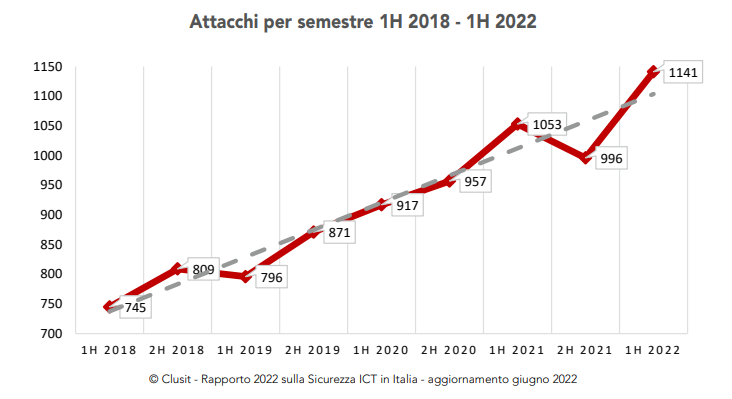
\includegraphics[scale=0.8]{Immagini/img1.png}
    \caption{Attacchi per semestre}
    \label{fig:AttacchiSemestre}
\end{figure}

Si può anche osservare la distribuzione mensile degli attacchi registrati nel primo semestre del 2022.

\begin{figure}[H]
    \centering
    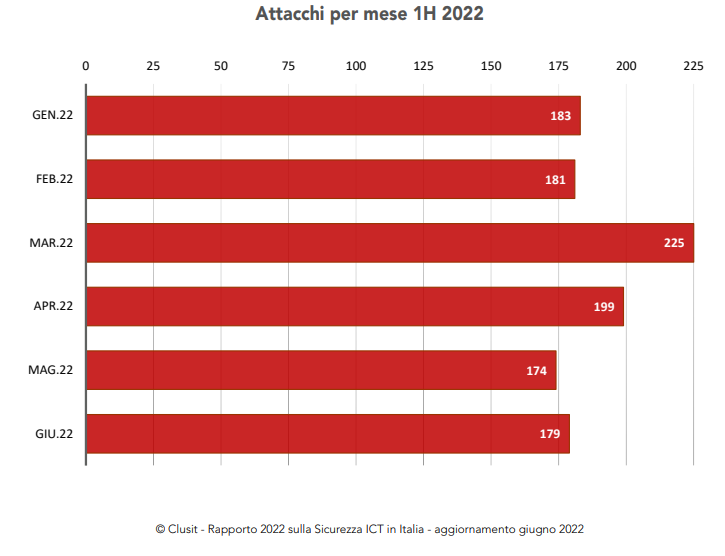
\includegraphics[scale=0.8]{Immagini/img2.png}
    \caption{Attacchi mensili}
    \label{fig:AttacchiMensili}
\end{figure}

Da questi dati si può iniziare ad evincere la gravità della situazione, in continuo peggioramento.

Le analisi e i relativi commenti si riferiscono ad un campione necessariamente parziale, per quanto ormai corposo e statisticamente significativo, rispetto al numero degli attacchi gravi effettivamente avvenuti nel periodo in esame. Questo accade sia perché un buon numero di aggressioni non diventano mai di dominio pubblico, oppure lo diventano ad anni di distanza (solitamente quanto più gli attacchi sono sofisticati), sia perché in molti casi è interesse delle vittime non pubblicizzare gli attacchi subiti, se non costretti dalle circostanze o da obblighi normativi particolari.

\chapter{Minacce note e classificazioni}
\section{Il concetto di malware}
Malware o “software malevolo” è un termine generico che descrive un programma/codice dannoso che mette a rischio un sistema. Ostili, invasivi e volutamente maligni, i malware cercano di invadere, danneggiare o disattivare computer, sistemi, reti, tablet e dispositivi mobili, spesso assumendo il controllo parziale delle operazioni del dispositivo. Lo scopo dei malware è riscuotere illecitamente a spese degli utenti. Sebbene i malware possono rubare, criptare o eliminare i dati, alterare o compromettere le funzioni fondamentali di un computer e spiare le attività degli utenti senza che questi se ne accorgano o forniscono alcuna autorizzazione, sono quindi anch’essi considerati veri e propri rischi. Per questa ragione è importante studiare e classificare i software malevoli, creando delle librerie di malware chiamate anche collezioni. Queste collezioni sono importantissime per il ricercatore che le utilizza per fare dei test su strumenti di sicurezza che dovrebbero riconoscerli ( come gli antivirus ) per sistematizzare tutta la conoscenza.

Ci sono varie tipologie di malware in cui si potrebbe incombere: 
\begin{itemize}
    \item Gli adware sono software indesiderati progettati per presentare messaggi pubblicitari sullo schermo, spesso all'interno di un browser web. Generalmente, gli adware si avvalgono di un metodo subdolo, mascherandosi da componenti legittimi o nascondendosi in un altro programma al fine di provocarne con l'inganno l'installazione su PC, tablet o dispositivo mobile.
    \item Gli spyware sono malware che osservano segretamente le attività dell'utente sul computer, senza autorizzazione, per poi segnalarle al creatore del software.
    \item I virus sono malware che si attaccano ad altri programmi e, quando eseguiti, di solito inavvertitamente, si riproducono modificando altri programmi e infettandoli con il proprio codice.
    \item I worm sono malware simili ai virus, che si riproducono per diffondersi sugli altri computer di una rete e danneggiandoli, di solito, mediante la distruzione di dati e file.
    \item Un trojan o "cavallo di Troia" è uno dei malware più pericolosi. Di solito si presenta sotto forma di qualcosa di utile, per ingannare l'utente. Una volta entrato nel sistema, i criminali ottengono l'accesso non autorizzato al computer della vittima. Da qui, i trojan possono essere utilizzati per rubare dati finanziari o installare altre minacce, come virus e ransomware.
    \item I ransomware sono malware che impediscono all'utente di accedere al proprio dispositivo e/o criptano i suoi file, obbligandolo a pagare un riscatto per riottenerli. I ransomware sono stati definiti "l'arma scelta" dei criminali, perché richiedono un pagamento rapido e ingente in criptovalute difficili da rintracciare. Il codice alla base dei ransomware è semplice da ottenere sui marketplace criminali e difendersi da essi è molto difficile.
    \item I rootkit sono dei malware che forniscono al criminale i privilegi da amministratore del sistema infetto. Generalmente, sono progettati per rimanere nascosti agli occhi dell'utente, degli altri software e del sistema operativo stesso.
    \item I keylogger sono malware che registrano la pressione dei tasti degli utenti sulla tastiera, memorizzando le informazioni raccolte e inviandole ai criminali responsabili, che puntano a informazioni sensibili come nomi utente, password o dati delle carte di credito.
    \item Il cryptomining dannoso, noto anche come drive-by mining o cryptojacking, è una tecnica malware sempre più diffusa, che in genere prevede l'installazione da parte di un trojan. Consente a persone estranee di utilizzare un computer per "generare" (mining) criptovalute, ad es. Bitcoin o Monero. Anziché lasciare che gli utenti raccolgano i frutti del lavoro del proprio computer, i cryptominer inviano la valuta raccolta ai propri account. Essenzialmente, un cryptominer dannoso deruba gli utenti delle loro risorse per lucro.
\end{itemize}
\subsection{Come proteggersi dai malware}
Presentiamo in seguito delle best practice da seguire per prevenire un attacco malware:
\begin{itemize}
    \item Prestare particolare attenzione ai domini che finiscono con strane combinazioni di lettere, ossia in qualcosa di diverso da com, org, edu o biz, per dirne alcuni, poiché possono indicare la pericolosità di un sito web.
    \item Non fare clic su pop-up pubblicitari mentre si naviga su internet. Non aprire allegati e-mail non richiesti o scaricare software da siti web affidabili.
    \item Assicurarsi che il sistema operativo, i browser e i plugin che utilizzi siano sempre aggiornati.
    \item Non scaricare app da terze parti.
    \item Non fare clic sui link non verificati contenuti in e-mail, SMS e messaggi di origine sconosciuta.
    \item Fare uso di un buon programma anti-malware. 
\end{itemize}
\subsection{Attacchi Malware recenti}
Uno degli attacchi ransomware più recenti è avvenuto all'inizio di gennaio  2023 a Yum! Questo attacco ha causato la chiusura di 300 punti vendita dei suoi marchi KFC, Pizza Hut e Taco Bell.  
\cite{Malware}
Questo attacco ransomware sembra essere stata una doppia estorsione che ha messo a rischio il furto di database, dati riservati e sistemi dell'operatore del marchio.
\section{Attacchi DDoS}
\cite{attaccoDDOS}
Un attacco DDoS (Distributed Denial of Service) è un tentativo ostile di bloccare il normale traffico di un server, servizio o rete sopraffacendo la vittima o l’infrastruttura circostante inondandola di traffico Internet.
La conseguenza più comune di un attacco DDoS è che un sito o un servizio diventi improvvisamente lento o non disponibile. 
\subsection{Attacchi DDoS recenti}
Ad oggi, il più grande attacco DDoS è avvenuto nel settembre del 2017. L'attacco era diretto ai servizi di Google e ha raggiunto una dimensione di 2,54 Tbps. Gli aggressori hanno inviato pacchetti spoofed a 180.000 server Web, che a loro volta hanno inviato risposte a Google. L'attacco non è stato un incidente isolato: negli ultimi sei mesi gli aggressori avevano diretto più attacchi DDoS all'infrastruttura di Google.
\section{Attacchi zero-day}
\cite{attaccoZeroDay}
Gli attacchi zero-day, noti anche come exploit zero-day, sono tentativi riusciti da parte dei criminali informatici di trovare e sfruttare vulnerabilità del software fino a quel momento sconosciute. Sfortunatamente, in tutto il software sono presenti punti deboli che offrono backdoor sfruttabili dagli hacker per inserire malware o violare i dati. Gli attacchi che sfruttano vulnerabilità precedentemente sconosciute dagli ingegneri software sono chiamati attacchi "zero day" proprio perché gli sviluppatori hanno avuto a disposizione zero giorni per risolvere il problema prima dell'attacco.
Gli attacchi zero-day sono violazioni della sicurezza particolarmente pericolose proprio perché la loro estensione è sconosciuta. In risposta a un attacco, uno sviluppatore di software può creare una patch, che però non è di alcun aiuto per gli utenti già colpiti.

A peggiorare le cose, molti sistemi antivirus tradizionali utilizzano strumenti di rilevamento delle minacce che si basano sul trovare una corrispondenza tra firme rivelatrici e attacchi informatici noti. Poiché gli attacchi zero-day sfruttano vulnerabilità precedentemente sconosciute (e forse malware non ancora noti), non solo possono rimanere inosservati per lunghi periodi di tempo, ma è anche molto più difficile difendersi.
\subsection{Attacchi zero-day recenti}
\cite{attaccoZeroDayRecente}
Uno degli attacchi Zero-day più recenti è stato ritrovato nel sistema operativo CISCO IOS XE. Si tratta di Privilege Escalation ed è stimato un attacco grave dal momento che se sfruttata la vulnerabilità da parte di un utente malintenzionato non autenticato, permette ad esso la creazione di un account di tipo admin dall’interfaccia Web UI e riuscirebbe ad ottenere il controllo dei dispositivi target.
\section{Vulnerabilità web e come classificarle} 
\cite{MITRE&CVE}
\cite{CVE}
MITRE Corporation: in pochi anni il MITRE è diventato un riferimento per la Cybersecurity. Tra i più significativi risultati vi è la creazione del database delle CVE (Common Vulnerability Explosure), un programma per identificare, definire e catalogare la vulnerabilità conosciute dei software che possono creare problematiche di sicurezza.Gli ottimi risultati di questo lavoro sono sfociati nel framework MITRE ATT\&CK: un archivio globale di tutte le tecniche e le tattiche di attacco derivate dall’osservazione e dalla studio delle compromissioni che hanno avuto successo.
CVE: Il Common Vulnerabilities and Exposures (in italiano Vulnerabilità ed esposizioni comuni), è un dizionario di vulnerabilità e falle di sicurezza note pubblicamente. Le vulnerabilità,sono identificate da un identificatore univoco che permette una maggiore comunicazione nel mondo della sicurezza e aiuta nella valutazione della diffusione di servizi e strumenti. Gli identificatori delle CVE prevedono:
\begin{itemize}
    \item CVE Id: composto da CVE, anno e numero sequenziale
    \item breve descrizione della vulnerabilità
    \item ogni altro riferimento utile 
\end{itemize}
\cite{rischiodigitale}
CWE: il CWE, ovvero Common Weakness Enumeration, è un elenco sviluppato dalla comunità di utenti di tipi di debolezze del software (commerciale o open source) e dell’hardware. Serve come linguaggio comune, metro per gli strumenti di sicurezza del software e base per l’identificazione delle debolezze, le mitigazioni e gli sforzi di prevenzione. Il CWE offre una tassonomia delle vulnerabilità suddividendole in circa 700 categorie tra cui: buffer overflow, path/directory tree traversal error, race condition, cross-site scripting, hard-coded password e insecure random number.
CAPEC: il Common Attack Pattern Enumeration and Classification fornisce un catalogo pubblicamente disponibile di modelli di attacco comuni che aiuta gli utenti a capire come gli avversari sfruttano i punti deboli nelle applicazioni.
Ogni modello di attacco acquisisce informazioni su come vengono progettate ed eseguite parti specifiche di un attacco e fornisce indicazioni sui modi per mitigare l'efficacia dell'attacco. I modelli di attacco aiutano coloro che sviluppano applicazioni a comprendere meglio gli elementi specifici di un attacco e come impedirne il successo.
OWASP è un’iniziativa open-source internazionale no-profit nata nel 2001 con lo scopo di realizzare una serie di linee guida ma anche di strumenti pratici, utili a supportare i web developer nello sviluppo sicuro di web application.
Trattandosi di un progetto open source, tutte le risorse messe a disposizione della community sono liberamente consultabili da chiunque voglia mettere la sicurezza al centro del suo progetto di sviluppo.

Le tecniche e i principi definiti da OWASP stanno diventando delle best practices riconosciute a livello internazionale per la prevenzione delle vulnerabilità informatiche.

Tramite l’applicazione sistematica di queste procedure lo sviluppatore può ridurre considerevolmente il rischio di data breach (violazione/perdita di dati) causati da attacchi hacker e agevolati da una scarsa qualità del codice.
Si tratta per il momento di indicazioni facoltative, ma in diversi contesti si sta cercando di renderle obbligatorie per lo sviluppo web.

Un passo in avanti in questo senso si è avuto con l’adozione del GDPR (Regolamento generale per la protezione dei dati personali) che richiede il rispetto della protezione dei dati fin dalla progettazione di un software, secondo il principio di privacy by design.
\subsection{Ultimi cambiamenti top10} 
\cite{Top10}
Ci sono tre nuove categorie nella Top 10 per il 2021, si possono qui vedere i cambiamenti e le differenze tra la top 10 stilata nel 2017 e la top 10 del 2021.
Subito sotto verranno riportate le descrizioni di ogni categoria illustrata della sola versione più recente.
\begin{figure}[H]
    \centering
    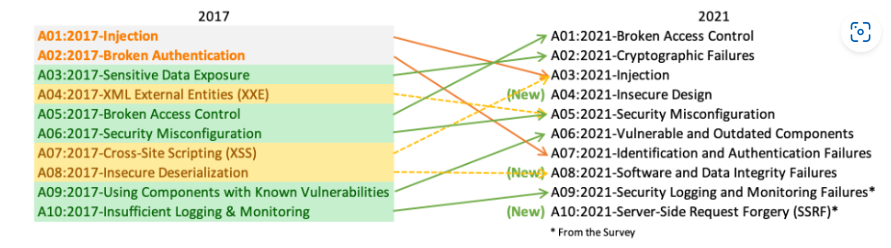
\includegraphics[scale=0.8]{Immagini/img3.png}
    \caption{Cambiamenti top10}
    \label{fig:cambiamentiTop10}
\end{figure}
\subsection{Broken Access Control} 
Il controllo degli accessi fa rispettare la policy in modo che gli utenti non possano agire al di fuori dei permessi previsti. Problematiche su questo tipo di controllo tipicamente portano alla divulgazione non autorizzata di informazioni, alla modifica o alla distruzione di tutti i dati o l'esecuzione di una funzione di business al di fuori dei limiti dell'utente. 
\subsection{Come prevenire Broken Access Control}
Il controllo degli accessi è efficace solo nel codice lato server o API server-less, dove l'attaccante non può modificare i meccanismi di controllo dell'accesso o i metadati.

\begin{itemize}
    \item Tranne che per le risorse pubbliche, applicare il principio di deny by default.
    \item Implementare i meccanismi di controllo dell'accesso una volta sola e utilizzarli in tutta l'applicazione, incluso limitare l'utilizzo di Cross-Origin Resource Sharing (CORS).
    \item I controlli di accesso del Model dovrebbero imporre la proprietà dei record piuttosto che accettare che l'utente possa creare, leggere, aggiornare o cancellare qualsiasi record.
    \item I requisiti unici dei vincoli di business di un'applicazione dovrebbero essere applicati nei modelli di dominio.
    \item Disabilitare il directory listing del server web e garantire che i metadati dei file (ad es, .git) e i file di backup non siano presenti all'interno delle web roots.
    \item Registrare i fallimenti dei meccanismi di controllo dell'accesso, avvisare gli amministratori quando appropriato (ad es, fallimenti ripetuti).
    \item Implementare meccanismi di rate limiting per accesso all'API e al controller per minimizzare il danno da strumenti di attacco automatizzati.
    \item Gli identificatori di sessione stateful dovrebbero essere invalidati sul server dopo il logout. I token JWT stateless dovrebbero piuttosto essere di breve durata in modo che la finestra di opportunità per un attaccante sia ridotta al minimo. Per i JWT di lunga durata è altamente raccomandato di seguire gli standard OAuth per revocare l'accesso.
\end{itemize}

Gli sviluppatori e lo staff di QA dovrebbero includere test funzionali di controllo dell'accesso e test di integrazione.
\subsection{Cryptographic Failures} 
Il primo passo è determinare le esigenze di protezione dei dati. Per esempio, password, numeri di carte di credito, documenti sanitari, informazioni personali e segreti aziendali richiedono una protezione adeguata, soprattutto se quei dati ricadono sotto le leggi sulla privacy, ad es. General Data Protection Regulation (GDPR), o regolamenti, ad es, protezione dei dati finanziari come il PCI Data Security Standard (PCI DSS). 

Per tutte queste tipologie di dati bisogna porre maggiore attenzione nel momento in cui: i dati sono trasmessi in chiaro,  sono implementati algoritmi o protocolli crittografici vecchi o deboli,  sono utilizzate chiavi crittografiche deboli, vecchie e/o riutilizzate, non viene applicata adeguata crittografia, le password sono chiavi crittografiche, vengono utilizzate funzioni hash deprecate. 
\subsection{Come prevenire Cryptographic Failures} 
\begin{itemize}
    \item Identificare quali dati sono sensibili secondo le leggi sulla privacy, requisiti normativi o esigenze aziendali.
    \item Non conservare inutilmente i dati sensibili. Eliminarli il prima possibile.
    \item Assicurarsi di cifrare tutti i dati sensibili a riposo.
    \item Utilizzare algoritmi, protocolli e chiavi standard forti e aggiornati. Avere un adeguato processo di key management.
    \item Crittografare tutti i dati in transito con protocolli sicuri come TLS con cifrari che garantiscano la FS (forward secrecy).
    \item Disabilitare il caching per le risposte che contengono dati sensibili.
    \item Usare sempre un meccanismo di crittografia autenticata invece della semplice crittografia.
    \item Evitare funzioni crittografiche e schemi di padding deprecati
    \item Assicuratevi che la randomness crittografica venga utilizzata laddove appropriato, e che non sia stato utilizzato un seed prevedibile o con bassa entropia.  
\end{itemize}
\subsection{Injection} 
Una applicazione è vulnerabile alle injection quando i dati forniti dall’utente non sono validati, filtrati o sanificati, le query dinamiche senza escaping contestuale vengono passate direttamente all’interprete, input malevolo viene utilizzato in modo diretto o concatenato. 

Le forme più comuni di injection che si possono trovare sono: SQL, NoSQL, OS command (quando il payload inserito dall'utente malintenzionato viene eseguito come comando del sistema operativo), Expression Language (quando l’attaccante controlla i dati in entrata dell’interprete). Questi risultano solo alcuni attacchi injection ma ce ne possono essere di molte altre tipologie.
\subsection{Come prevenire Injection} 
\begin{itemize}
    \item Per qualsiasi query dinamica è consigliabile svolgere l'escape dei caratteri speciali usando la sintassi di escape specifica per quell’interprete.
    \item Usare controlli SQL all’interno delle query per prevenire la divulgazione di massa dei record, questo in caso di SQL injection.
    \item Utilizzare validazione degli input lato server.
    \item Per qualsiasi query dinamica è consigliabile svolgere l'escape dei caratteri speciali usando la sintassi di escape specifica per quell’interprete.
    \item Usare controlli SQL all’interno delle query per prevenire la divulgazione di massa dei record, questo in caso di SQL injection.
\end{itemize}
\subsection{Insecure Design}
Insecure Design viene definita come una macro categoria che include tutte le problematiche legate alla progettazione inefficace o mancante dei controlli di sicurezza in un’infrastruttura web-based. Negli ultimi decenni, quest’area d’indagine ha visto grandi progressi grazie soprattutto al continuo incremento degli attacchi informatici a danno delle infrastrutture web-based e cloud-based.

Quando si parla di design insicuro di un’applicazione web si fa riferimento ad una infrastruttura costruita su basi non solide: le vulnerabilità si trovano nel codice sorgente. Al contrario quando si parla di difetti di implementazione software parliamo di una struttura di base sicura ma che viene aggiornata con pezzi di codice che comportano la comparsa di vulnerabilità a lungo termine. 

La progettazione insicura di un software o di implementazione in ogni caso, comportano una serie di pericoli che sono provocati dal trascurare gli standard di sicurezza informatica minimi. Ad ogni modo, la presenza di vulnerabilità di InSecure Design costituisce un problema non da poco considerato che le minacce informatiche sono in continua evoluzione e risolvere queste problematiche significa riprogettare logiche e funzionamenti del software.
\subsection{Come prevenire Insecure Design} 
\begin{itemize}
    \item Stabilire e utilizzare un ciclo di vita di sviluppo sicuro con i professionisti di AppSec per aiutare a valutare e progettare la sicurezza e i controlli relativi alla privacy.
    \item Stabilire e utilizzare una libreria di design pattern sicuri o componenti pronti all'uso.
    \item Integrare i controlli di plausibilità ad ogni livello della vostra applicazione (dal frontend al backend).
    \item Scrivere test unitari e di integrazione per convalidare che tutti i flussi critici siano resistenti al modello di minaccia rappresentato. Compilare i casi d'uso e i casi di uso improprio per ogni livello della vostra applicazione.
    \item Limitare il consumo di risorse per utente o servizio.  
\end{itemize}
\subsection{Security Misconfiguration}
Una applicazione potrebbe risultare vulnerabile se ci sono permessi configurati in maniera impropria sui servizi cloud, se sono abilitate o installate funzioni non necessarie, se account di default sono ancora abilitati con password predefinite, a seguito di condizione di errore vengono rivelati agli utenti messaggi di errore verbosi, se nei sistemi aggiornati le funzionalità di sicurezza non vengono abilitate o configurate nella maniera opportuna, se le impostazioni di sicurezza non sono configurati in maniera consona su valori sicuri e/o se  il software non è aggiornato.
\subsection{Come prevenire Security Misconfiguration}
\begin{itemize}
    \item Un processo di hardening (insieme di operazioni specifiche di configurazione di un dato sistema informatico che mira a minimizzare l’impatto di possibili attacchi informatici) ripetibile rende veloce e facile il deploy ( è il processo di installazione, configurazione, aggiornamento ed abilitazione di un’applicazione o di una suite di applicazioni che consente di utilizzare un sistema software ) di un altro ambiente preconfigurato in modo sicuro. Gli ambienti di sviluppo dovrebbero essere tutti configurati in modo speculare, con credenziali diverse per ogni ambiente. Questo processo dovrebbe essere automatizzato per minimizzare lo sforzo richiesto per impostare un nuovo ambiente configurato in modo sicuro.
    \item Rimuovere o non installare funzionalità e framework inutilizzati.
    \item Inserire un task per rivedere ed aggiornare le configurazioni appropriate a tutte le security notes.
    \item L'invio di direttive di sicurezza ai client, ad esempio, i Security Headers.
    \item Un processo automatizzato per verificare l'efficacia delle configurazioni e impostazioni in tutti gli ambienti.
\end{itemize}
\subsection{Vulnerable and Outdated Components}
La vulnerabilità si presenta nel caso in cui il software risulta vulnerabile, non supportato o non aggiornato, se non si fa la scansione delle vulnerabilità di libreria regolarmente e non si consultano i report di sicurezza relativi ai componenti utilizzati, se non si corregge/aggiorna la piattaforma sottostante, i framework, le dipendenze in maniera tempestiva, se gli sviluppatori non testano la compatibilità delle librerie aggiornate o delle librerie nuove o se i componenti non vengono configurati in modo sicuro.
\subsection{Come prevenire Vulnerable and Outdated Components}
Per prevenire questa tipologia di vulnerabilità bisognerebbe: 

\begin{itemize}
    \item Rimuovere le dipendenze, le funzionalità, i componenti, i file, e la documentazione non utilizzate.
    \item Inventariare in modo continuo le versioni dei componenti lato client e lato server (ad esempio, framework, librerie) e le loro dipendenze usando strumenti come OWASP.
    \item Monitorare continuamente fonti come Common Vulnerability and Exposures (CVE) e il National Vulnerability Database (NVD) per vulnerabilità nei componenti.
    \item Ottenere i componenti solo da fonti ufficiali tramite link sicuri. Preferire pacchetti firmati per ridurre la possibilità di includere un componente modificato o dannoso.
    \item Controllare le librerie e i componenti che non sono più mantenuti o che non sviluppano più patch di sicurezza per le vecchie versioni. Se il patching non è possibile, considerare l'implementazione di una patch virtuale per monitorare, rilevare o proteggere dal problema individuato.
\end{itemize}

\subsection{Identification and Authentication Failures}
Precedentemente sotto il nome di Broken Authentication ci possono essere debolezze sui meccanismi di autenticazione nel caso in cui l’applicazione permette attacchi automatici dove l’attaccante ha una lista di coppie nome utente e password validi, se permette attacchi di brute force o altri attacchi automatici, se permette password di default deboli, se presenta un recupero delle credenziali e delle password deboli, se memorizza le password in chiaro, se non ha un sistema di autenticazione a due fattori, se riutilizza l’identificatore di sessione dopo un login avvenuto con successo, non l’indicatore di sessione.
\subsection{Come prevenire Identification and Authentication Failures}
Per prevenire questa tipologia di vulnerabilità bisognerebbe: 

\begin{itemize}
    \item Implementare l'autenticazione a più fattori per prevenire attacchi di credential stuffing, brute force e riutilizzo delle credenziali rubate.
    \item Non mettere in produzione sistemi con credenziali di default, in particolare per gli utenti admin.
    \item Implementare controlli sulla debolezza delle password, come verificare le password nuove o modificate con la lista delle 10,000 password peggiori.
    \item Allineare i requisiti di lunghezza delle password, complessità e politiche di rotazione con le linee guida della sezione 5.1.1 del documento 800-63b pubblicato dal National Institute of Standards and Technology (NIST) riguardante la memorizzazione dei secret o altre policy relative alle password moderne.
    \item Limitare o ritardare sempre più i tentativi di login falliti, ma fare attenzione a non creare uno scenario di denial of service. Loggare tutti i tentativi falliti e avvertire gli amministratori quando vengono rilevati attacchi di credential stuffing, brute force o altri.
\end{itemize}

\subsubsection{Autenticazione a due fattori}
\cite{Autenticazione2fattori}
Al giorno d’oggi non risulta più sufficiente proteggere i propri account con password forti, è consigliabile utilizzare una autenticazione forte conosciuta come autenticazione a due fattori. 

Risulta ormai noto l’importanza di utilizzare password molto complesse e diverse, come allo stesso tempo utilizzare strumenti per riuscire a ricordare tutte le password che ci ritroviamo a gestire. Per risolvere questa problematica si utilizzano dei password manager, applicazioni che hanno la funzione di mantenere le nostre password in maniera crittografata. 

Tutto questo però non basta a garantire la sicurezza di una password, in generale una autenticazione basata sull’utilizzo di una sola password risulta debole. 

Per questa motivazione è stata introdotta l’autenticazione a due fattori che rappresenta uno dei sistemi per mantenere al sicuro i nostri dati. 

Solitamente l’autenticazione può avvenire in diversi modi: 
\begin{itemize}
    \item Conoscenza: una cosa che sai (password o PIN)
    \item Possesso: una cosa che hai (smarthphone o token di sicurezza)
    \item Inerenza: una cosa che sei (impronte digitale, timbro vocale etc..)
\end{itemize}
L’autenticazione a due fattori avviene nel momento in cui si utilizzano due dei tre fattori sopra elencati. 

Solitamente nell’autenticazione a due fattori in seguito all’inserimento della password verrà richiesto un secondo fattore. 

Risulta indispensabile che il secondo fattore sia inattaccabile, in caso contrario il problema dell’effettuare una autenticazione sicura non sarebbe risolto. 

Grazie all’affinarsi delle tecniche di hacking mediante Intelligenza artificiale e il deepfake che consente di imitare volti e voci, la cyber security in senso ampio viene messa in difficoltà, è dunque sconsigliato l’utilizzo di Inerenza.

Da linee guida del NIST si consiglia quindi di ottenere il  secondo fattore attraverso lo smartphone (sotto forma di sms o tramite un’apposita applicazione) o tramite un token fisico perché generato in maniera pseudocasuale secondo uno specifico algoritmo ed ha una durata molto limitata nel tempo (solitamente 30 secondi).  Per questo motivo, lo si definisce anche OTP: “one time password”.

Acronimo di “One-Time-Password”, le OTP sono password che possono essere usate una sola volta e questo, già da solo, costituisce una garanzia in più rispetto alle password tradizionali, sempre identiche e utilizzabili per un periodo di tempo variabile a seconda delle policy aziendali. Le OTP sono una combinazione di caratteri numerici o alfanumerici più difficili da violare perché possono essere usate una sola volta e, di norma almeno, vengono inviate a un dispositivo in dotazione all’utente.
Esistono due tipologie di OTP utilizzabili:
\begin{itemize}
    \item TOTP, password monouso valide per un periodo limitato di tempo solitamente per 15-60 secondi. Una volta scaduto il tempo assegnato, il codice non è più utilizzabile ed è necessaria l’assegnazione di uno nuovo. Più la vita del codice è breve, più è difficile violarlo perché una persona non autorizzata deve ottenere il codice in un lasso di tempo ristretto.  
    \item HOTP, password monouso basate su HMAC, ossia un codice di autenticazione che fa leva su una funzione di hash. Mediante HMAC sono garantite l’integrità e l’autenticità di un messaggio, è una metodologia quasi non più utilizzata. 
\end{itemize}

\subsection{Software and Data Integrity Failures}
Le problematiche dell'integrità del software e dei dati riguardano il codice e l'infrastruttura che non ne verificano adeguatamente l'integrità. Un esempio è quando un'applicazione si affida a plugin, librerie o moduli da fonti, repository e content delivery network (CDN) non attendibili.
\subsection{Come prevenire Software and Data Integrity Failures}
\begin{itemize}
    \item Usare firme digitali o meccanismi equivalenti per verificare che il software o i dati provengano dalla fonte prevista e non siano stati alterati.
    \item Assicuratevi che venga usato uno strumento di sicurezza della supply chain del software, come OWASP Dependency Check o OWASP CycloneDX, per verificare che i componenti non contengano vulnerabilità note.
    \item Assicurarsi che ci sia un processo di revisione per le modifiche al codice e alla configurazione per ridurre al minimo la possibilità che codice o configurazione dannosi vengano introdotti nella pipeline del software.
    \item Assicurarsi che la pipeline CI/CD sia adeguatamente segregata, configurata adeguatamente e sia presente un meccanismo di controllo degli accessi per assicurare l'integrità del codice che passa attraverso i processi di compilazione e distribuzione.
    \item Assicuratevi che i dati serializzati non firmati o non crittografati non vengano inviati ai client non fidati senza qualche forma di controllo dell'integrità o firma digitale per rilevare la manomissione o il replay dei dati serializzati.  
\end{itemize}
\subsection{Security Logging and Monitoring Failures}
Questa categoria è per aiutare a rilevare, svolgere escalation e rispondere alle violazioni attive. Senza logging e monitoraggio, le violazioni non possono essere rilevate. Il logging, il rilevamento, il monitoraggio e la risposta attiva insufficienti si verificano ogni volta che gli eventi verificabili come il login, i login falliti e le transazioni ad alto valore non vengono registrate, se warning ed errori sono inadeguati/poco chiari, se i file di log vengono memorizzati solo localmente, se non sono presenti le soglie di allarme/processi di escalation della risposta, i penetration test e le scansioni non danno nessun allarme, se l’applicazione non è in grado di rilevare, svolgere escalation o avvisare per gli attacchi attivi in real-time o quasi real time. Si è poi inoltre vulnerabili alla fuga di informazioni se gli eventi di logging e gli alert sono visibili ad un utente o ad un attaccante.
\subsection{Come prevenire Security Logging and Monitoring Failure}
\begin{itemize}
    \item Assicurarsi che tutti i login, il controllo degli accessi e gli errori a seguito della verifica degli input lato server possono essere registrati con un contesto utente sufficiente per identificare account sospetti o malevoli e conservati per un tempo sufficiente a consentire un'analisi forense a posteriori.
    \item Assicurarsi che i dati di log siano codificati correttamente per prevenire injection o attacchi ai sistemi di registrazione o monitoraggio.
    \item Assicurarsi che le transazioni di alto valore abbiano un audit trail con controlli di integrità per prevenire manomissioni o cancellazioni, come le tabelle append-only di un database, o simili.
    \item I team DevSecOps dovrebbero stabilire sistemi di monitoraggio di allerta efficaci in modo che le attività sospette siano rilevate e affrontate rapidamente.
    \item Stabilire o adottare un piano incident response e recovery, come ad esempio il National Institute of Standards and Technology (NIST) 800-61r2 o successivo.
\end{itemize}
\subsection{Server-Side Request Forgery}
Le falle SSRF si verificano ogni volta che un'applicazione web recupera una risorsa remota senza validare l'URL fornito dall'utente. Questo permette ad un attaccante di forzare l'applicazione ad inviare una richiesta preparata ad hoc ad una destinazione inattesa, anche quando è protetta da un firewall, una VPN o un altro tipo di network access control list (ACL).

Dato che le moderne applicazioni web forniscono agli utenti finali parecchie funzionalità, scaricare dati da un URL è uno scenario comune. Di conseguenza, l'incidenza di SSRF è in crescita. Inoltre, la gravità di SSRF sta diventando più alta a causa dei servizi cloud e alla complessità crescente delle architetture.
\subsection{Come prevenire Server-Side Request Forgery}
\subsubsection{Dal layer di rete:}
\begin{itemize}
    \item Segmentare in reti separate le funzionalità che richiedono un accesso alle risorse remote per ridurre l'impatto di SSRF.
    \item Applicare politiche di firewall "deny by default" o regole di controllo per bloccare tutto il traffico intranet tranne quello essenziale.
\end{itemize}
\subsubsection{Dal layer applicativo:}
\begin{itemize}
    \item Sanitizzare e convalidare tutti i dati di input forniti dal cliente.
    \item Far rispettare lo URL schema, la porta e la destinazione con una allow list
    \item Non inviare risposte raw ai client.
\end{itemize}
\subsubsection{Praticità}
Non mitigare la SSRF attraverso l'uso di una deny list o di un'espressione regolare. Gli attaccanti hanno a disposizione liste di payload, strumenti e abilità per bypassare le deny list.
\section{Standard , best practice e leggi }
\subsection{Il GDPR}
\subsubsection{Terminologia utile}
Verrà in seguito riportata la terminologia necessaria per poter comprendere a fondo i concetti riportati.

Dato personale:per dato personale si intende “qualsiasi informazione relativa a persona fisica identificata o identificabile (data subject); una persona identificabile è una persona che può essere identificata, direttamente o indirettamente, in particolare mediante riferimento a un numero di identificazione o a uno o più fattori propri della sua identità fisica, fisiologica, psichica, economica, culturale o sociale".

Trattamento dei dati personali: per trattamento dei dati personali si intende tutto il processo che parte dall’acquisizione dei dati, comprende la modalità di utilizzo dei dati stessi, la conservazione, fino alla cancellazione 

Titolare del trattamento: il titolare è la persona fisica, l'autorità pubblica, l'impresa, l'ente pubblico o privato, l'associazione che adotta le decisioni sugli scopi e sulle modalità del trattamento

Violazione dei dati personali: una violazione (accidentale o malevola) della sicurezza che porta alla distruzione, perdita, alterazione, divulgazione o accesso non autorizzati ai dati personali trasmessi, archiviati o altrimenti trattati
\subsubsection{Introduzione}
\cite{gdpr}
\cite{gdpr2}
Il Regolamento UE 679/2016 (noto come GDPR, acronimo di “General Data Protection Regulation”) ha introdotto una disciplina uniforme e armonizzata a livello comunitario per la protezione delle persone fisiche nel trattamento dei dati.
Seppure si parli comunemente di “protezione dei dati”, il bene giuridico protetto è la
persona fisica. Quindi tutta la disciplina va letta, interpretata e applicata tenendo conto
che l’obiettivo è proteggere le persone dai danni che potrebbero derivare da un non corretto trattamento dei dati.
Il GDPR deve essere applicato da coloro che trattano dati personali, con solo alcune
eccezioni riportate nell’articolo 2 del Regolamento medesimo.
\subsubsection{La rilevanza giuridica dell’analisi del rischio}
Il GDPR chiede al titolare del trattamento di analizzare il rischio a cui i dati sono sottoposti e di identificare le misure di gestione e sicurezza idonee a eliminarlo o mitigarlo.
\subsubsection{Adempimenti per l’analisi del rischio}
\begin{itemize}
    \item Liceità, correttezza e trasparenza: le organizzazioni devono assicurarsi che le loro attività di raccolta dati personali degli utenti non infrangano la  legge e che non nascondano nulla agli interessati. Per fare ciò, è necessario mettere a disposizione del pubblico l’informativa sulla privacy, ossia un documento che spiega in maniera chiara, concisa ma completa le finalità della raccolta dei dati e come l’azienda intenda usarli. 
    \item Limitazione della finalità: Le aziende dovrebbero raccogliere i dati personali solamente per uno scopo preciso, scopo che va indicato in modo chiaro nell’informativa sulla privacy. Inoltre, tali dati vanno tenuti solo per il tempo necessario a completare lo scopo per cui sono stati raccolti.
    \item Minimizzazione dei dati: Le organizzazioni possono elaborare solo i dati personali necessari al raggiungimento della finalità per i quali sono trattati.
    \item Esattezza: L’accuratezza dei dati personali è parte integrante della loro protezione. Il GDPR afferma che “devono essere adottate tutte le misure ragionevoli per cancellare o rettificare tempestivamente i dati inesatti”. Gli interessati hanno il diritto di chiedere che i propri dati personali inesatti o incompleti vengano cancellati o rettificati.
    
    Una volta che il titolare o il responsabile del trattamento ha ricevuto tale richiesta da parte dell’interessato, ha 30 giorni di tempo per eseguirla.
    \item Limitazione della conservazione:le organizzazioni devono eliminare i dati personali quando non sono più necessari ai propri scopi.
    \item Integrità e riservatezza: Il GDPR afferma che i dati personali devono essere “trattati in maniera da garantire un’adeguata sicurezza dei dati personali, compresa la protezione, mediante misure tecniche e organizzative adeguate, da trattamenti non autorizzati o illeciti e dalla perdita, dalla distruzione o dal danno accidentali”.
    
    Nonostante ciò, il Regolamento è abbastanza vago sulle misure di sicurezza da implementare. Attualmente, le organizzazioni ricorrono alla crittografia e alla pseudonimizzazione dei dati dove possibile, ma potrebbero scegliere qualsiasi altra opzione disponibile più adatta ai propri scopi. 
    
\end{itemize}
\subsection{Il NIST}
\cite{NIST}
La stragrande maggioranza delle piccole imprese fa affidamento sulla tecnologia dell'informazione per gestire le proprie attività e archiviare, elaborare e trasmettere informazioni. Proteggere queste informazioni da divulgazione, modifica, utilizzo o cancellazione non autorizzati è essenziale per tali aziende e i loro clienti.

Proprio per questa ragione nasce nel 2013 il Cybersecurity Framework in seguito a un ordine esecutivo del Presidente degli Stati Uniti, nel quale veniva richiesto lo sviluppo di un’architettura per la cybersecurity da adottare su base volontaria, basato sulla gestione del rischio e che fosse “flessibile, ripetibile nell’applicazione, efficiente ed efficace a livello di costo di utilizzo e implementazione”.

Il framework offre un approccio flessibile alla gestione della cybersecurity, considerando gli asset fisici, informatici e le persone.
\subsubsection{Ambito di applicazione del NIST}
Pensato inizialmente per le sole infrastrutture critiche, è in realtà applicabile a ogni organizzazione che voglia meglio gestire il rischio di cybersicurezza.
\subsubsection{Architettura del framework}
La versione attuale è la 1.1 dell’aprile 2018, composta da cinque domini:
\begin{figure}[H]
    \centering
    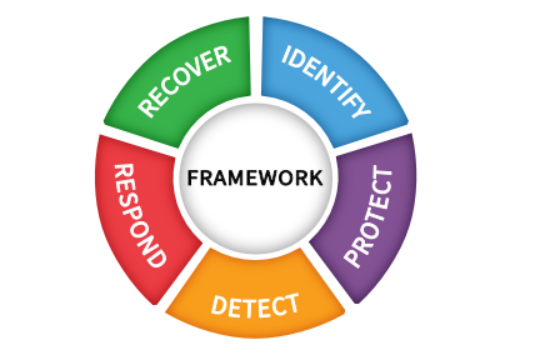
\includegraphics[scale=0.6]{Immagini/img4.png}
    \caption{Le 5 caratteristiche del NIST}
    \label{fig:caratteristicheNist}
\end{figure}
\begin{itemize}
    \item Identify (ID) – Conoscenza relativa ai sistemi, tecnologie, informazioni e le altre risorse e capacità che devono essere protette; definizione delle priorità di intervento in relazione alla strategia e missione dell’organizzazione; definizione dei processi atti a perseguire gli obiettivi definiti per mezzo dell’analisi dei rischi.
    \item Protect (PR) – Sviluppo e attuazione di appropriati presidi al fine di garantire l’erogazione dei servizi.
    \item Detect (DE) – Sviluppo e attuazione di appropriate attività deputate alla rilevazione e identificazione di eventi di sicurezza informatica.
    \item Respond (RS) – Pianificazione, sviluppo e attuazione di appropriate attività di reazione a un evento di sicurezza informatica identificato e rilevato.
    \item Recover (RC) - Sviluppo e attuazione di appropriate attività atte a ripristinare le risorse e capacità che sono state compromesse da un evento di sicurezza informatica.
\end{itemize}
Ogni dominio è suddiviso in categorie (categories), ossia gruppi di attività deputate a specifici e definiti obiettivi di sicurezza informatica, e sotto-categorie, specifiche e dettagliate attività aventi natura tecnica o manageriale. Ogni sottocategoria a sua volta prevede micro-attività a livello di obiettivo da raggiungere.

Si può osservare in seguito una tabella che rappresenta lo scenario descritto sopra con le varie attività specificate:

\begin{figure}[H]
    \centering
    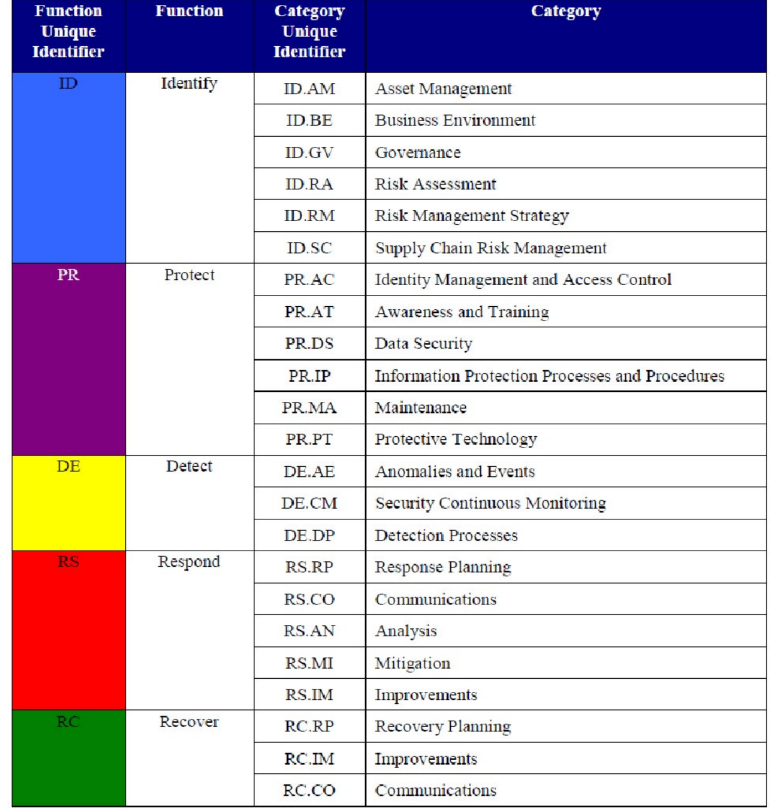
\includegraphics[scale=0.8]{Immagini/img5.png}
    \caption{Tabella riassuntiva caratteristiche NIST}
    \label{fig:caratteristicheRiassuntiveNIST}
\end{figure}


\chapter{La valutazione del rischio digitale}
\section{Risk assessment e risk management }
La valutazione dei rischi digitali è fondamentale per le organizzazioni che intendono
avere la piena consapevolezza della loro situazione e desiderino affrontare un percorso
di miglioramento continuo. Formalmente, l’analisi del rischio (risk analysis) è parte della
valutazione del rischio (risk assessment), a sua volta parte della gestione del rischio
(risk management). Quest’ultima è organizzata in più fasi interconnesse: 
\begin{figure}[H]
    \centering
    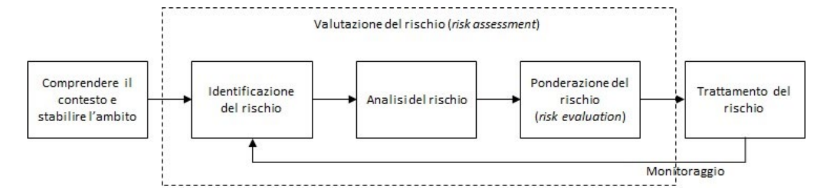
\includegraphics[scale=0.9]{Immagini/img6.png}
    \caption{Valutazione del rischio}
    \label{fig:ValutazioneRischio}
\end{figure}

Alcuni testi indicano come “gestione del rischio” la sola fase di trattamento del rischio.
L’approccio deve essere sistematico, ossia tale da rendere evidente, e quindi ripetibile, attraverso i dati, le elaborazioni e le valutazioni, il ragionamento che ha portato alle scelte fatte. Questo permette anche di verificare, validare e affinare nel tempo il proprio approccio alla gestione del rischio, riducendo conseguentemente l’aleatorietà delle valutazioni fatte.

I principali passi della gestione del rischio consistono in: 
\begin{itemize}
    \item Comprensione del contesto e stabilire l’ambito:
        \begin{itemize}
            \item Analisi del contesto: consente di cogliere tutti gli elementi che contribuiscono allo sviluppo di una conoscenza del rischio e di adattare il processo di analisi del rischio alle effettive esigenze del settore di attività.
            \item Identificazione dell’approccio da adottare e dei framework di riferimento: la scelta dell’approccio da adottare rende la gestione del rischio pertinente, inquadrando gli elementi più significativi e prendendo in considerazione tutti i tipi di rischi applicabili alle attività e funzioni. L’adozione di un framework permette di stabilire un dizionario di termini e misure condivise con tutti.  
            \item Mappatura dei processi, inclusa la filiera di fornitura:  costituisce il punto di partenza per una descrizione dettagliata dell’attività dell’organizzazione e, quindi, per l’identificazione delle aree e attività più critiche. 
            \item Identificazione del perimetro da analizzare.
            \item Assegnazione delle responsabilità: l’individuazione puntuale dei risk owner intesi come persone responsabili dell’analisi delle minacce e delle vulnerabilità in specifici ambiti e, conseguentemente, della gestione del rischio anche nelle attività quotidiane. Devono avere i necessari poteri per attuare le adeguate misure di mitigazione dei rischi e interagire con i vertici e le persone incaricate del coordinamento complessivo della gestione dei rischi.
        \end{itemize}   
    \item Valutazione del rischio:  identificazione e caratterizzazione dei pericoli e dell’esposizione a essi, quantificazione del rischio, in relazione alle minacce esistenti e alla probabilità che queste possano concretizzarsi, e valutazione della sua accettabilità in relazione al contesto e alle strategie dell’organizzazione. Si divide in:
        \begin{itemize}
            \item identificazione del rischio: Il metodo per identificare le vulnerabilità, conosciute (ed elencate nel CVE) e sconosciute, di un sistema è il cosiddetto Vulnerability Assessment (VA).  Possiamo suddividere VA in 4 fasi:
                \begin{itemize}
                    \item La prima fase prevede un vulnerability scanning, eseguito con strumenti automatici di scansione delle vulnerabilità ; esso permette di individuare una buona parte delle vulnerabilità già note.
                    \item La seconda fase prevede un security test evaluation (STE), con il quale si svolgono dei test di base tesi alla ricerca delle vulnerabilità più semplici.
                    \item Successivamente si eseguono penetration test (PT) effettuati da persone con elevate competenze tecniche.
                \end{itemize}
            \item analisi del rischio:  l’esecuzione di un’analisi dei rischi è un’attività ricca di incognite, sia per quanto concerne la sua conduzione, sia per quanto attiene i risultati ottenuti. È quindi particolarmente importante che si abbia consapevolezza di questi limiti: ci possono essere errori negli approcci utilizzati, la conoscenza imperfetta della minaccia, nuove vulnerabilità da scoprire (etc.. ) e per questa motivazione dovrebbero essere adeguatamente documentate le scelte e gli approcci effettuati.
            \item ponderazione dei rischi: confronto del livello di rischio residuo con i criteri di accettazione condivisi con i vertici dell’organizzazione.
        \end{itemize}
    \item Trattamento dei rischi: valutazione delle alternative disponibili per affrontare il rischio (per esempio, mitigandolo o accettandolo).
    \item Riesame del rischio (risk monitoring and review):  attività in cui sono raccolte e analizzate informazioni relative ai rischi in modo da verificare l’efficacia del loro trattamento. 
\end{itemize}
\section{Integrazione continua DevSecOps}
\cite{DevSecOps}
\cite{DevSecOps2}
DevSecOps è una pratica di integrazione dei test di sicurezza in ogni fase del processo di sviluppo del software chiamato DevOps. 

DevOps utilizza strumenti e automazione per promuovere una maggiore collaborazione, comunicazione e trasparenza tra team.

La Continuous Integration and Continuous Delivery (CI/CD) è una moderna pratica di sviluppo software che utilizza passaggi automatizzati di compilazione e test per fornire in modo affidabile ed efficiente piccole modifiche all'applicazione. Gli sviluppatori utilizzano gli strumenti CI/CD per rilasciare nuove versioni di un'applicazione.

Include strumenti e processi che incoraggiano la collaborazione tra sviluppatori, specialisti della sicurezza e team operativi per creare software efficiente e sicuro. DevSecOps porta una trasformazione culturale che rende la sicurezza una responsabilità condivisa per tutti coloro che stanno costruendo il software. DevSecOps introduce la sicurezza nella pratica DevOps integrando le valutazioni della sicurezza in tutto il processo CI/CD. Rende la sicurezza una responsabilità condivisa tra tutti i membri del team coinvolti nella creazione del software.
\subsection{Vantaggi DevSecOps}
L’impiego della metodologia DevSecOps consente di rilasciare software migliore in maniera più veloce, identificando nativamente le possibili vulnerabilità che potrebbero dare luogo a seri problemi in seguito ai deploy pianificati lungo la roadmap dell’applicazione.
\subsection{Pipeline DevSecOps} 
Le pipeline DevSecOps, conosciute anche come pipeline CI/CD, consistono in una successione di script eseguiti in sequenza per la realizzazione di una nuova versione del software. L'introduzione di monitoraggio e automazione mira a potenziare lo sviluppo, il testing e il rilascio dell'applicativo. Pur essendo possibile eseguire ogni passaggio manualmente, l'integrazione all'interno di una pipeline garantisce un processo più rapido ed efficiente.

I passaggi che costituiscono una pipeline CI/CD sono una serie di attività raggruppate in ciò che è noto come fase della pipeline. Le fasi tipiche della pipeline includono:

\begin{itemize}
    \item Build: si compila l’applicazione e si testano le funzionalità.
    \item Test: in questa fase si eseguono i test di sicurezza. 
    \item   Release: in questa fase il codice viene rilasciato in ambiente di testing.
\end{itemize}
Se vengono con successo le precedenti fasi citate,  avverrà il deploy in produzione.
Ecco un esempio in cui si effettua il deploy, successivamente potremmo osservare il fallimento di alcuni di questi campi.
\begin{figure}[H]
    %centrare senza margini
    \makebox[\textwidth][c]{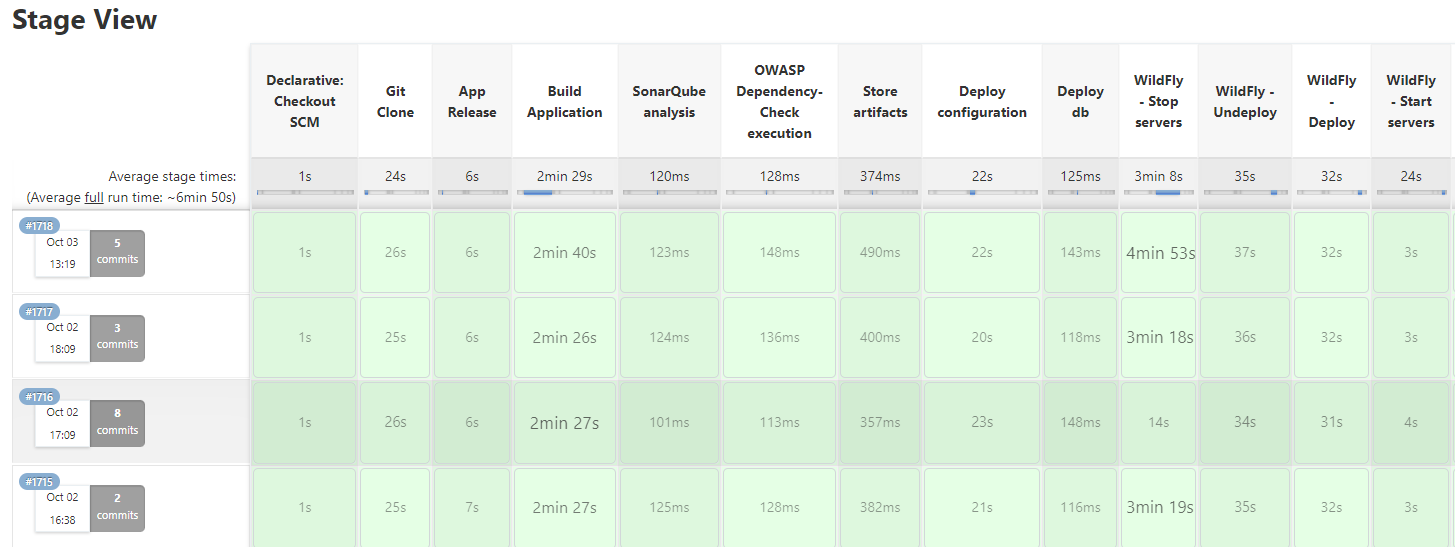
\includegraphics[scale=0.55]{Immagini/img7.png}}%
    \caption{Pipeline di successo}
    \label{fig:pipelineSuc}
\end{figure}
In questa immagine riportata sopra possiamo osservare queste diverse fasi testate dai plugin scaricati dall’applicazione utilizzata che verrà analizzata in seguito.
\section{Analisi dei report}
Alcuni strumenti che esamineremo offriranno agli utenti la possibilità di generare report al fine di segnalare ogni tipo di possibile pericolo individuato.

Il processo coinvolge scansioni automatizzate e la valutazione delle vulnerabilità presenti in un sistema, con l'obiettivo di individuare e correggere potenziali punti deboli che potrebbero essere sfruttati da un attaccante.

L'inizio del processo consiste nelle scansioni automatizzate del sistema, utilizzando strumenti software specializzati noti come Vulnerability Scanner. Questi scanner esaminano il sistema alla ricerca di vulnerabilità, come falle di sicurezza nel sistema operativo, applicazioni web, database, firewall e altri componenti del sistema.

Dopo il completamento della scansione, il Vulnerability Scanner prosegue con la valutazione delle vulnerabilità individuate per determinarne la gravità e il rischio associato. Tale valutazione si basa su metriche standard come il Common Vulnerability Scoring System (CVSS), che classifica le vulnerabilità in base alla loro gravità e alla loro rilevanza per l'organizzazione.

Per ogni vulnerabilità individuata, è disponibile una dettagliata descrizione, il livello di rischio, la localizzazione precisa della vulnerabilità e le indicazioni per risolvere il problema.

Il compito del pentester consiste nel verificare la validità delle segnalazioni. Se una segnalazione è valida, il problema deve essere corretto; in caso contrario, la vulnerabilità individuata può essere dichiarata erroneamente positiva.
\section{Tecnologie DevSecOps}
Analogamente ai progetti basati su DevOps, l'utilizzo di strumenti DevSecOps richiede un'automazione completa, limitando, in casi eccezionali, qualsiasi intervento manuale e evitando modifiche alle configurazioni e script personalizzati. 

Gli strumenti DevSecOps devono garantire una risposta in tempo reale, poiché la velocità dei cicli CI/CD e la riduzione del time to market delle applicazioni rimangono tra i principali driver per l'adozione delle metodologie di sviluppo agili. Ottimizzare anche i requisiti di sicurezza dell'applicazione entro tempi ragionevoli costituisce un valore aggiunto fondamentale.

L'automazione e la velocità devono essere accompagnate da precisione e qualità, altrimenti i risultati del lavoro potrebbero essere compromessi da un'esperienza scadente causata da funzionalità sviluppate in modo inefficiente o, nella peggiore delle ipotesi, da sistemi instabili e affetti da bug.

Sul fronte della sicurezza, è cruciale limitare i falsi positivi e i falsi negativi, fenomeni che potrebbero rallentare drasticamente un'applicazione generando allarmi di sicurezza privi di fondamento. Una corretta implementazione di DevSecOps richiede che gli strumenti siano in grado di eseguire test di sicurezza per eliminare o ridurre al minimo gli allarmi dovuti a falsi positivi e falsi negativi, fornendo al team di sviluppo informazioni utili per correggere tempestivamente le vulnerabilità individuate.
\subsection{Jenkins}
\cite{Jenkins}
Jenkins è un server open source di CI/CD (Continuous Integration, Continuous Deployment) scritto in Java. 

Jenkins consente di automatizzare le diverse fasi del ciclo di vita del software, dalla compilazione al test alla distribuzione.

Una delle caratteristiche principali di Jenkins è la Jenkins Pipeline (o semplicemente "Pipeline") che è una suite di plug-in che supporta l'implementazione e l'integrazione di pipeline di distribuzione continua in Jenkins.

Una pipeline di distribuzione continua è un'espressione automatizzata del processo per ottenere il software dal controllo della versione fino ai tuoi utenti e clienti.

Jenkins Pipeline fornisce un set estendibile di strumenti per modellare pipeline di distribuzione da semplici a complesse. 

Le esecuzioni delle pipeline possono essere azionate in vari modi, tra cui un commit oppure ad ogni intervallo di tempo oppure attraverso l'interfaccia web. 

Inoltre le sue funzionalità possono essere potenziate dal grande numero di plug-in compatibili, sviluppati e diffusi dalla comunità di utenti e developer che lo usa.

Nel momento in cui si esegue si possono osservare le varie fasi di sviluppo build, test e release per poi passare alla fase di deploy. 

In seguito illustreremo delle pipeline di esecuzione in cui ci sarà un fallimento (pipeline senza fallimento vedere sopra). 
\begin{figure}[H]
    %centrare senza margini
    \makebox[\textwidth][c]{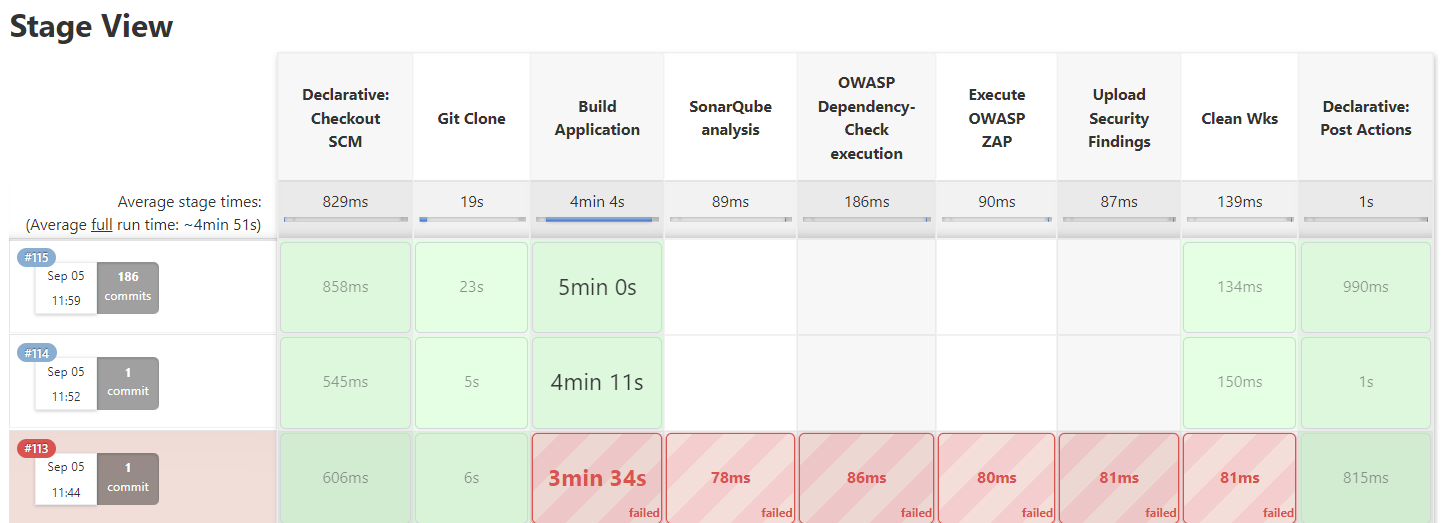
\includegraphics[scale=0.55]{Immagini/img8.png}}%
    \caption{Pipeline di fallimento}
    \label{fig:pipelineIns}
\end{figure}
Da questa immagine si può osservare un fallimento all’interno del processo di build che ha successivamente scatenato un fallimento un tutte le fasi successive. Il processo verrà quindi successivamente scartato.
\subsection{Snyk}
\cite{Snyk}
Snyk è una soluzione di sicurezza destinata agli sviluppatori che aiuta le aziende a usare il codice open source e consente di rimanere protetti. Basandosi sul suo esclusivo database di vulnerabilità, Snyk individua e corregge continuamente vulnerabilità note e violazioni delle licenze nelle dipendenze open source. Si integra nel flusso di lavoro degli sviluppatori e negli strumenti di controllo del codice sorgente (ad esempio GitHub, BitBucket, GitLab), agganciandosi alle pipeline CI/CD e monitorando continuamente Platform as a Service (PaaS) e app serverless in produzione.

La scansione altamente accurata di Snyk rileva le vulnerabilità in tempo reale e fornisce un contesto di definizione delle priorità olistico in modo da sapere sempre cosa risolvere per primo.

Snyk segnala ogni vulnerabilità trovata è popone modi di risoluzione del problema.
\begin{figure}[H]
    %centrare senza margini
    \makebox[\textwidth][c]{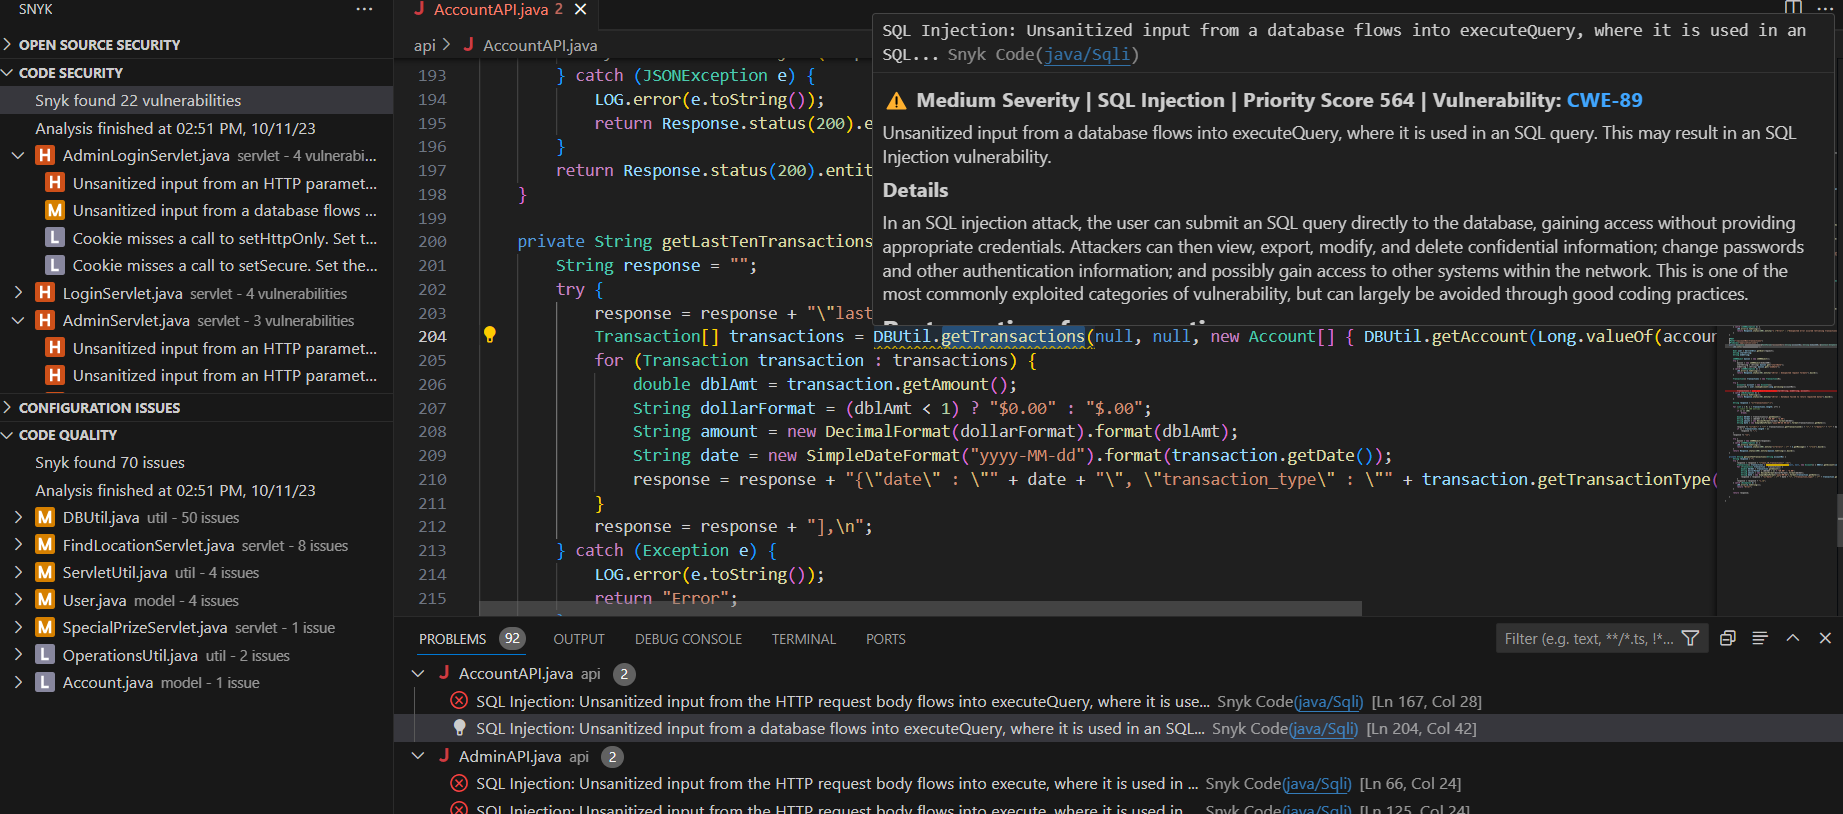
\includegraphics[scale=0.4]{Immagini/img9.png}}%
    \caption{Snyk Vulnerabilities}
    \label{fig:snyk}
\end{figure}
Come possiamo osservare in basso vengono segnalate tutte le vulnerabilità riscontrate. Selezionando una di quelle si aprirà la pagina esatta della vulnerabilità e selezionando il preciso contenuto vulnerabile si potranno visualizzare i dettagli precisi della vulnerabilità ed anche eventuali modi per risolverla.
\subsection{OWASP Dependency-Check} 
\cite{Dependency-Check}
Dependency check è uno strumento di analisi della composizione software che tenta di rilevare le vulnerabilità contenute nelle  dipendenze di un progetto. Il problema è che all’interno delle applicazioni si è soliti includere librerie di terze parti che potrebbero essere vulnerabili.

Come possiamo osservare dalla pipeline di sviluppo è uno degli aspetti da controllare all’interno del ciclo devsecops.
\subsection{Owasp ZAP} 
\cite{OWASP_ZAP}
OWASP Zed Attack Proxy (ZAP) è uno strumento di sicurezza che consente di rilevare vulnerabilità in applicazioni e siti Web. È una soluzione semplice e flessibile che si adatta a vari livelli di utilizzo e competenza. ZAP è composto da due macro-sezioni. La prima è uno scanner automatizzato di vulnerabilità che consente di identificare problemi e fornisce un report con i dettagli delle vulnerabilità per poter sanare la falla. La seconda permette a ZAP di operare come proxy che consente di ispezionare il traffico e tutta la comunicazione HTTP e gli eventi, con la possibilità di modificarli o analizzare i loro trigger che sono potenzialmente pericolosi per il sistema.

Viene riportato sotto un esempio dello scanner e del report associato ad esso.
\begin{figure}[H]
    %centrare senza margini
    \makebox[\textwidth][c]{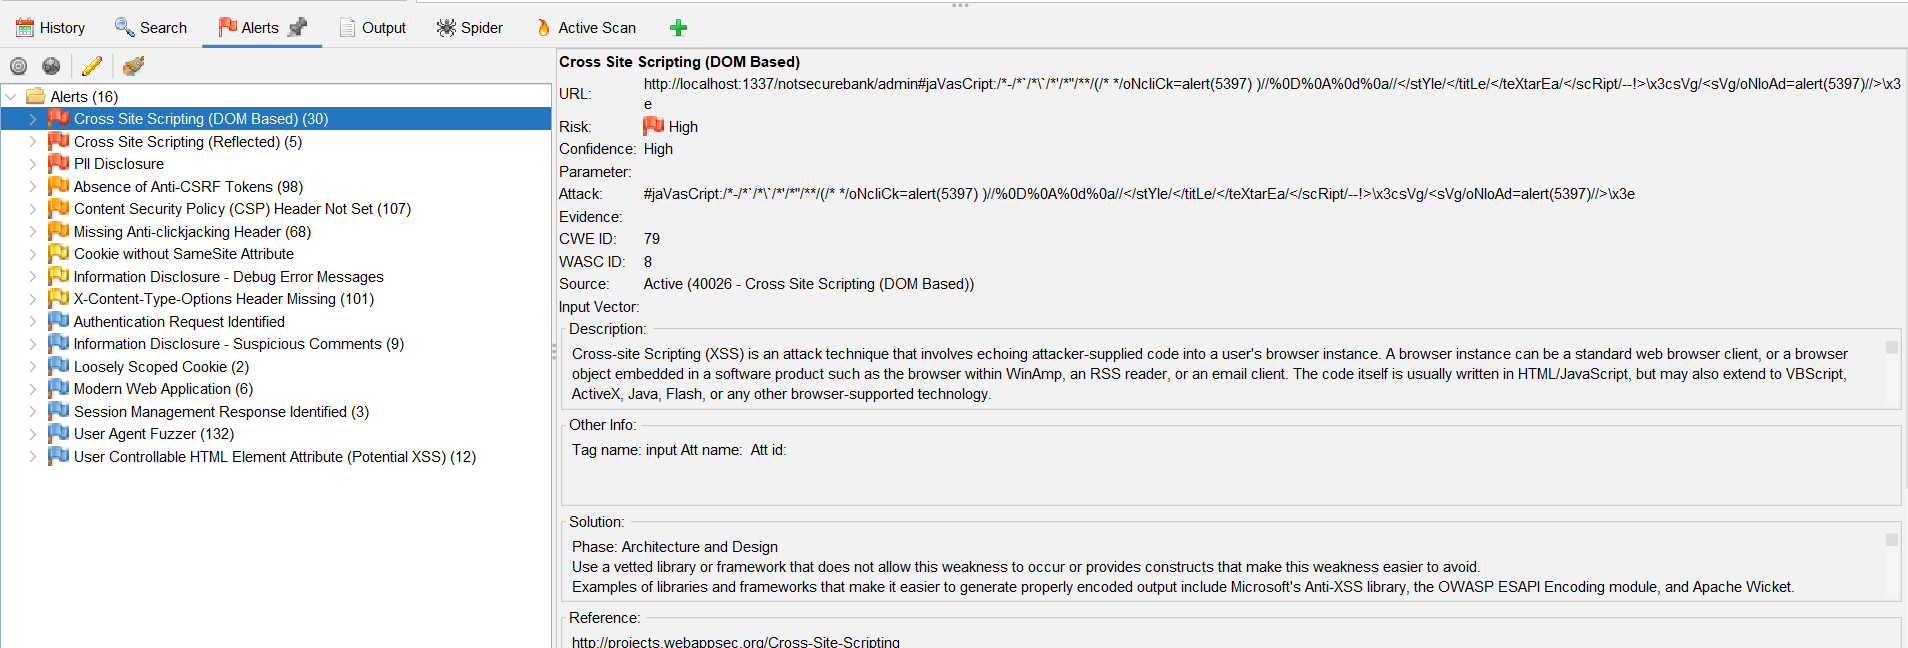
\includegraphics[scale=0.4]{Immagini/img12.png}}%
    \caption{Applicazione ZAP}
    \label{fig:zap}
\end{figure}
Come possiamo osservare sulla sinistra possiamo trovare la lista di tutte le vulnerabilità trovate, in ordine di criticità. Selezionando una di esse possiamo vedere dove si trova il problema, una descrizione dettagliata del problema ed uno dei modi di risoluzione. 

In questo modo una persona che esegue scanning avrà tutte le informazioni necessarie per verificare la problematica ed una volta verificata si potrà classificare come vulnerabilità o come falso positivo. 

Nella sicurezza informatica, si parla di falso positivo nel caso in cui si generi un allarme relativo ad un problema di cybersecurity che risulti però infondato. Ovvero nel caso in cui una minaccia viene rilevata e segnalata ma che in realtà non lo è.
\begin{figure}[H]
    %centrare senza margini
    \makebox[\textwidth][c]{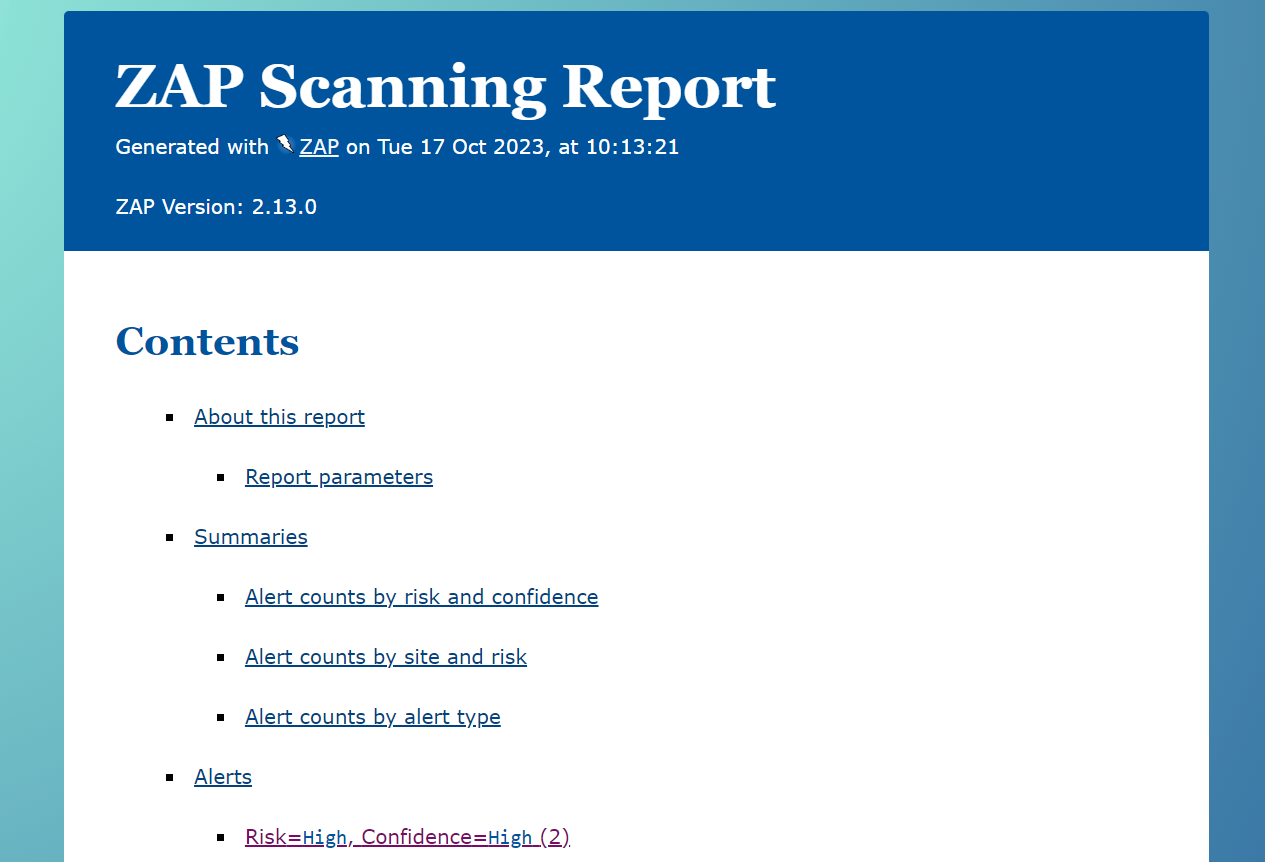
\includegraphics[scale=0.5]{Immagini/img11.png}}%
    \caption{ZAP report}
    \label{fig:report}
\end{figure}
Questa è una prima pagina di un report in cui troviamo l’indice di tale documento. Il documento sarà quindi formato da una prima parte introduttiva, una parte che comprende le statistiche e le valutazioni delle vulnerabilità riscontrate ed una parte finale in cui vengono illustrate una ad una le vulnerabilità. In questa ultima parte selezionando la vulnerabilità che si vuole analizzare si potrà trovare un link che porta direttamente alla pagina ufficiale della vulnerabilità OWASP. 
Offre dunque tutti gli strumenti necessari per poter effettuare una analisi dettagliata e completa delle vulnerabilità. 
\subsection{Esempi pratici} 
\subsubsection{Esempio di test di applicazioni java: Notsecurebank}
Motivazioni della scelta del linguaggio: Java è un linguaggio di programmazione orientata a oggetti multipiattaforma che viene eseguito su miliardi di dispositivi in tutto il mondo e nonostante sia stato creato più di 20 anni fa, java è attualmente il linguaggio più diffuso tra gli sviluppatori di App, ne citiamo qui alcune famose come per esempio Spotify,Twitter,LinkedIn e moltre altre. 

Spesso Java viene utilizzata con un framework come per esempio Spring che è molto diffuso per la creazione di applicazioni autonome, adatte ad ambienti di produzione che vengono eseguite su JVM. Java Spring Boot semplifica e velocizza lo sviluppo di applicazioni web. 

Di norma risulta vantaggioso utilizzare lo strumento Maven per i progetti Java, esso è in grado di organizzare le dipendenze facilitando l’organizzazione dei progetti in maniera più pulita standardizzando la sua struttura.

Nel nostro esempio utilizzeremo una semplice applicazione Java. 

Strumenti utilizzati:
\begin{itemize}
    \item Virtual machine NotSecureBank
    \item OWASP ZAP
\end{itemize}  
Virtual machine NotSecureBank:  è la macchina virtuale creata per l’applicazione vulnerabile che si vuole testare.
\begin{figure}[H]
    %centrare senza margini
    \makebox[\textwidth][c]{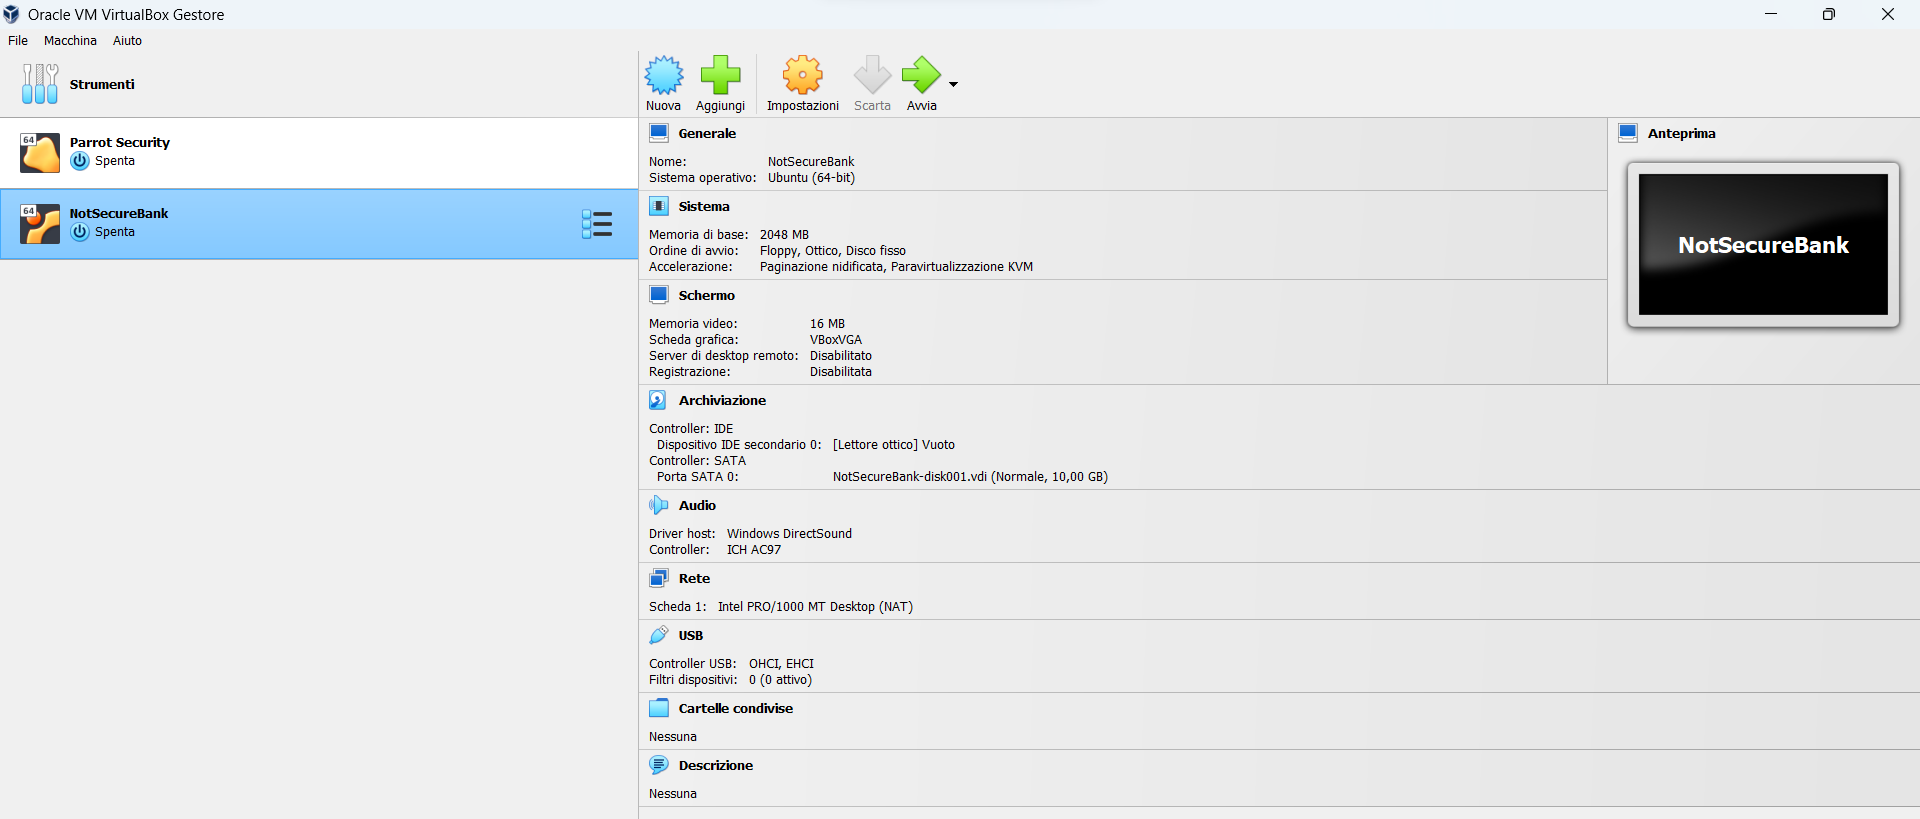
\includegraphics[scale=0.4]{Immagini/img13.png}}%
    \caption{Avvio Virtual machine NotSecureBank}
    \label{fig:avviovm}
\end{figure}
\begin{figure}[H]
    %centrare senza margini
    \makebox[\textwidth][c]{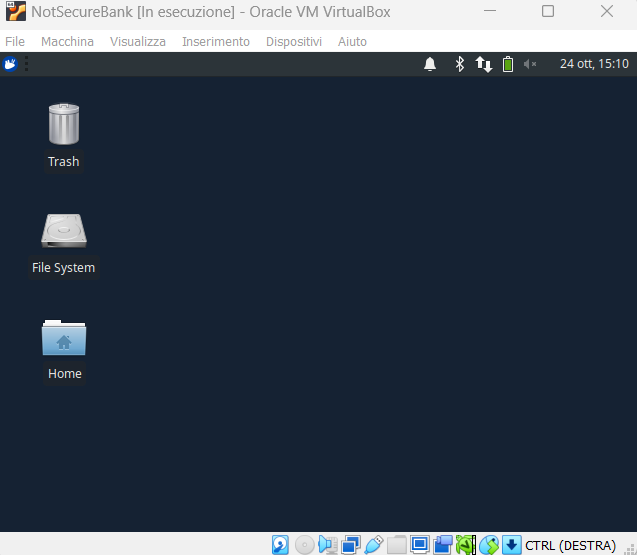
\includegraphics[scale=0.7]{Immagini/img14.png}}%
    \caption{Virtual machine NotSecureBank}
    \label{fig:vm}
\end{figure}
Una volta avviata la macchina NotSecureBank possiamo fare avviare una esecuzione automatica su Owasp zap all'indirizzo http://localhost:1337/notsecurebank a questo punto disponibile.

Viene visualizzato in seguito il risultato della scansione: 
\begin{figure}[H]
    %centrare senza margini
    \makebox[\textwidth][c]{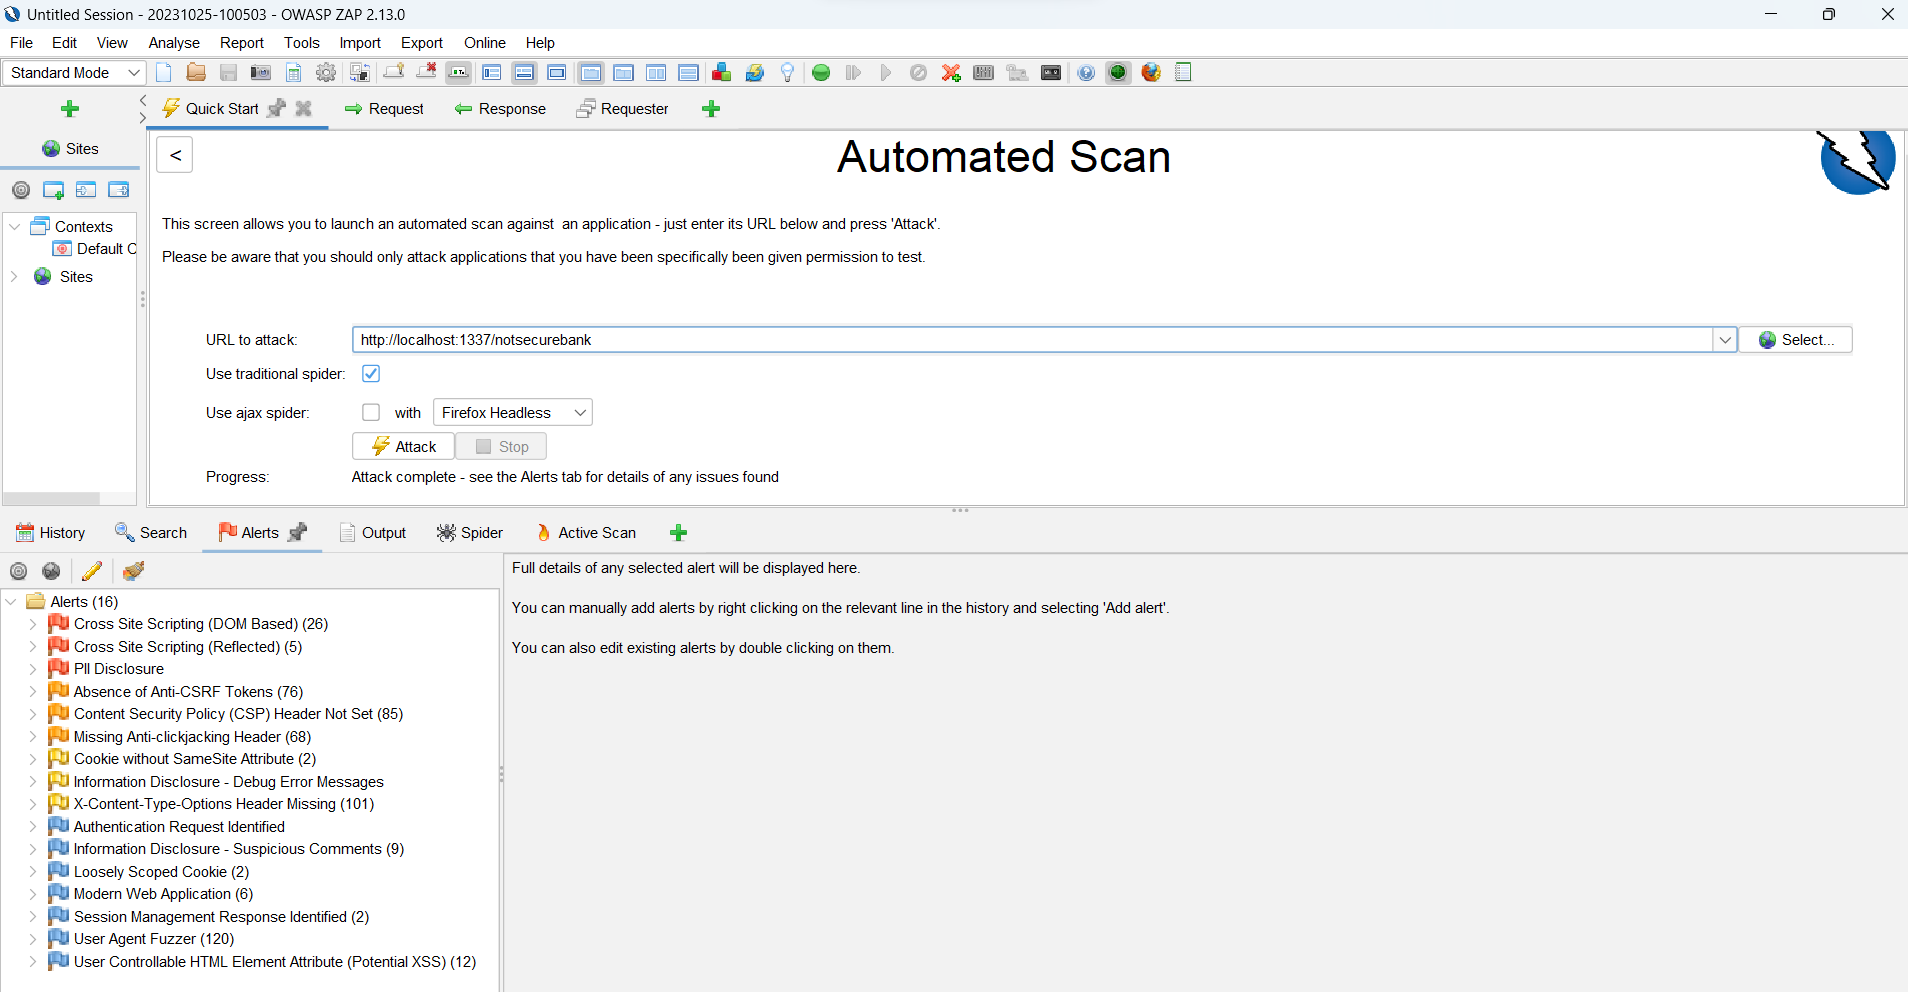
\includegraphics[scale=0.4]{Immagini/img10.png}}%
    \caption{Scanner Zap}
    \label{fig:scanzap}
\end{figure}
In basso a sinistra si trovano la lista di vulnerabilità trovate, dalla più grave alla meno grave, e selezionandole si potrà osservare la sua descrizione ed i modi per sanarla.
Per generare il report dell’analisi effettuata si dovrà cliccare sul pulsante in alto a destra e si otterrà in maniera automatica un report. 

Ecco la visualizzazione delle vulnerabilità all’interno del report:
\begin{figure}[H]
    %centrare senza margini
    \makebox[\textwidth][c]{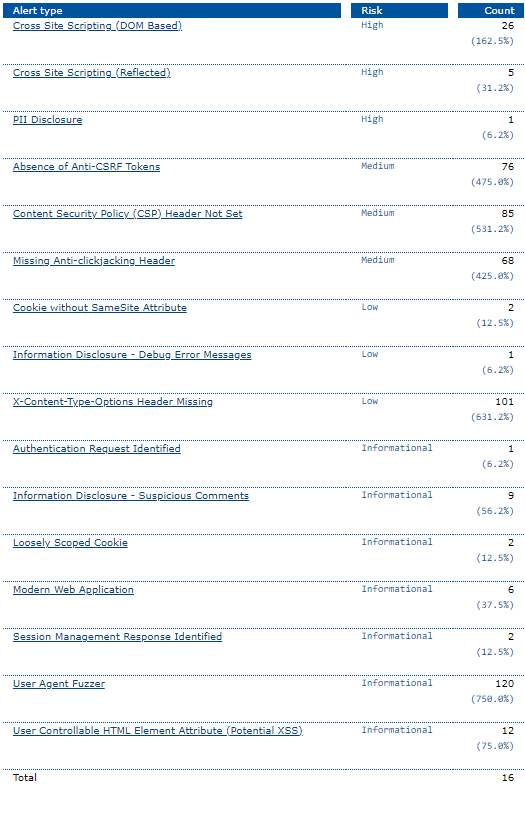
\includegraphics[scale=0.6]{Immagini/img15.png}}%
    \caption{Report finale NotSecureBank }
    \label{fig:reportNSB}
\end{figure}
Come possiamo osservare in questo report vengono riportate vere e proprie vulnerabilità e anche varie forme di pericolo, facilmente attaccabili e quindi segnalate.

Questo è solo un indice delle vulnerabilità e dei pericoli trovati, all’interno dell’intero report queste minacce verranno analizzate maggiormente nel dettaglio, descrivendo la vulnerabilità e come risolverla, inserendo riferimenti validi alla documentazione del problema stesso.

Di seguito alla generazione del report è opportuno testare manualmente le vulnerabilità trovate. 
\subsubsection{Esempio di test in angular}
Motivazioni sulla scelta del linguaggio: Angular è un framework di sviluppo web ampiamente utilizzato e apprezzato, che offre una vasta gamma di funzionalità e vantaggi per le aziende che desiderano creare applicazioni web dinamiche e interattive. Offre inoltre un ambiente di sviluppo solido e sicuro, riducendo al minimo gli errori e migliorando la manutenibilità del codice.
Eccone alcuni esempi: Netflix, PayPal e molte altre. 
Oltre ad Angular possono essere utilizzate delle tecnologie analoghe per modalità d’uso e funzionalità, le più utilizzate sono React e Vue. 

Questi framework o librerie, sono utilizzabili dopo l’installazione di Node.js che comprende NPM (Node Package Manager), il quale fornisce le dipendenze del progetto tramite configurazione, eventualmente riscontrando se ci sono vulnerabilità note all’interno del progetto. 

Ecco un esempio dell’installazione delle dipendenze del progetto: 
\begin{figure}[H]
    %centrare senza margini
    \makebox[\textwidth][c]{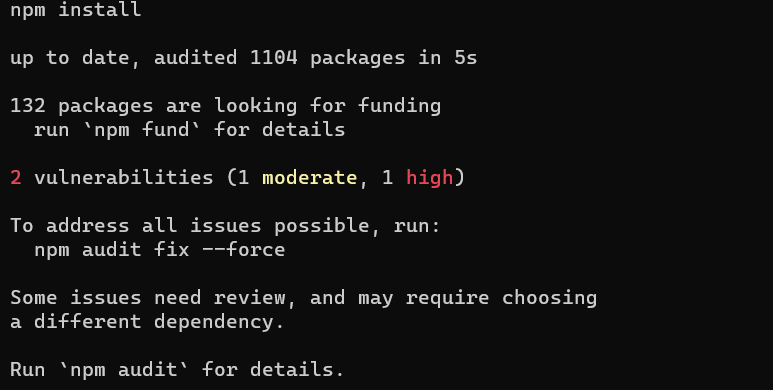
\includegraphics[scale=0.7]{Immagini/img16.png}}%
    \caption{Installazione npm }
    \label{fig:npmInstall}
\end{figure}
Si può osservare che (a differenza di un’installazione attraverso Maven) sono già state segnalate 2 vulnerabilità.
Per effettuare un’analisi delle vulnerabilità si utilizza il comando npm audit.
\begin{figure}[H]
    %centrare senza margini
    \makebox[\textwidth][c]{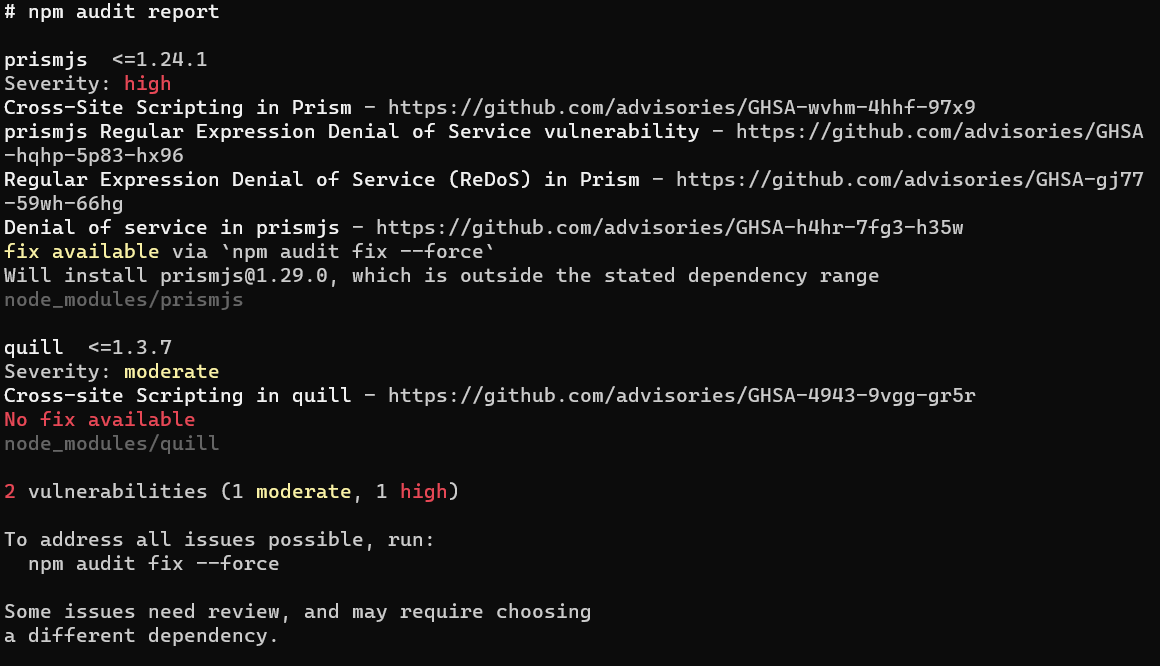
\includegraphics[scale=0.6]{Immagini/img17.png}}%
    \caption{npm audit }
    \label{fig:npmAudit}
\end{figure}
\begin{figure}[H]
    %centrare senza margini
    \makebox[\textwidth][c]{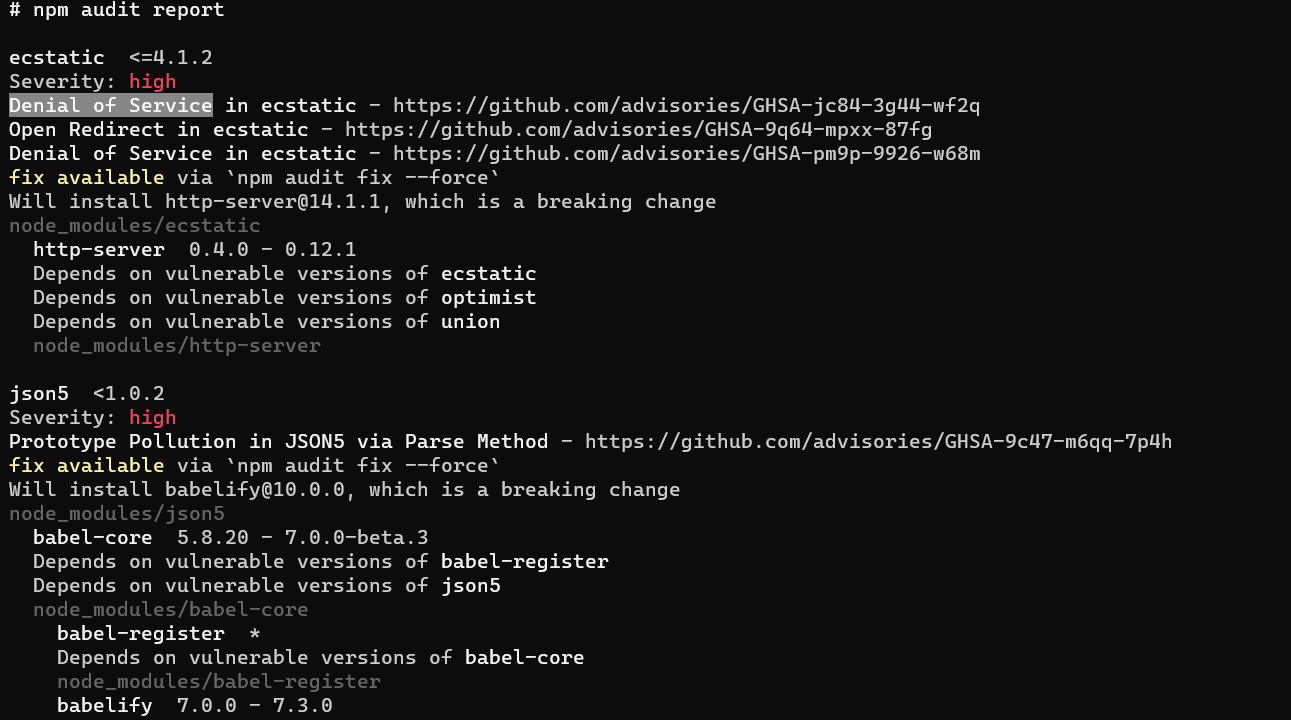
\includegraphics[scale=0.5]{Immagini/img18.png}}%
    \caption{Visualizzazione di vulnerabilità}
    \label{fig:viewVulnerability}
\end{figure}
Strumenti utilizzati:
\begin{itemize}
    \item Docker Desktop
    \item Progetto  github HackMEAN
    \item OWASP zap
\end{itemize}
Docker Desktop: Docker è un popolare software libero progettato per eseguire processi informatici in ambienti isolabili, minimali e facilmente distribuibili chiamati container Linux, con l'obiettivo di semplificare i processi di deployment di applicazioni software. Utilizzando i container le risorse possono essere isolate, i servizi limitati e i processi avviati in modo da avere una prospettiva completamente privata del sistema operativo, col loro proprio identificativo, file system e interfaccia di rete. I vantaggi di Docker si misurano in relazione alle macchine virtuali. Infatti, i container sono più leggeri delle macchine virtuali, vengono avviati più velocemente e richiedono meno risorse. 

Progetto  github HackMEAN: è una applicazione intenzionalmente vulnerabile costruita sullo stack MEAN (MongoDB, Express, Angular e Node.js). Questa applicazione illustra le vulnerabilità comuni nello stack MEAN. 
Il caso studio permette di trovare tutte le vulnerabilità eseguendo l'applicazione in uno scanner automatico e generarne il report associato.

Con l’utilizzo di docker, una volta scaricato il progetto ed aggiunto ai container,  è possibile avviare l’applicazione e una istanza mongodb in una volta sola.
\begin{figure}[H]
    %centrare senza margini
    \makebox[\textwidth][c]{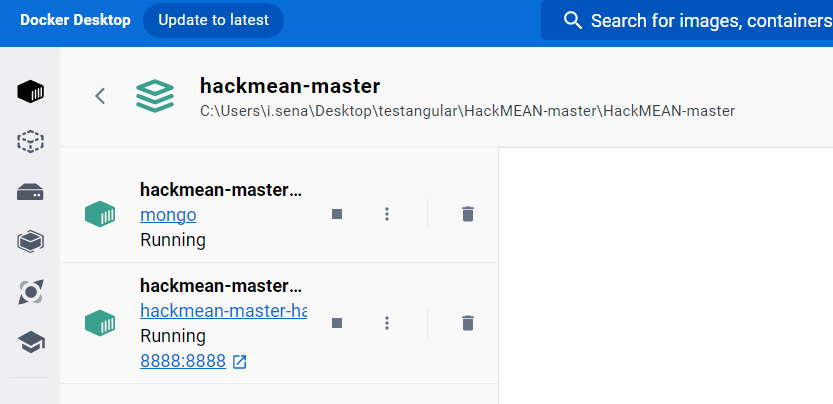
\includegraphics[scale=0.7]{Immagini/img19.png}}%
    \caption{Visualizzazione applicazione in Docker}
    \label{fig:Docker}
\end{figure}
In seguito verrà illustrata l’applicazione in esecuzione: 
\begin{figure}[H]
    %centrare senza margini
    \makebox[\textwidth][c]{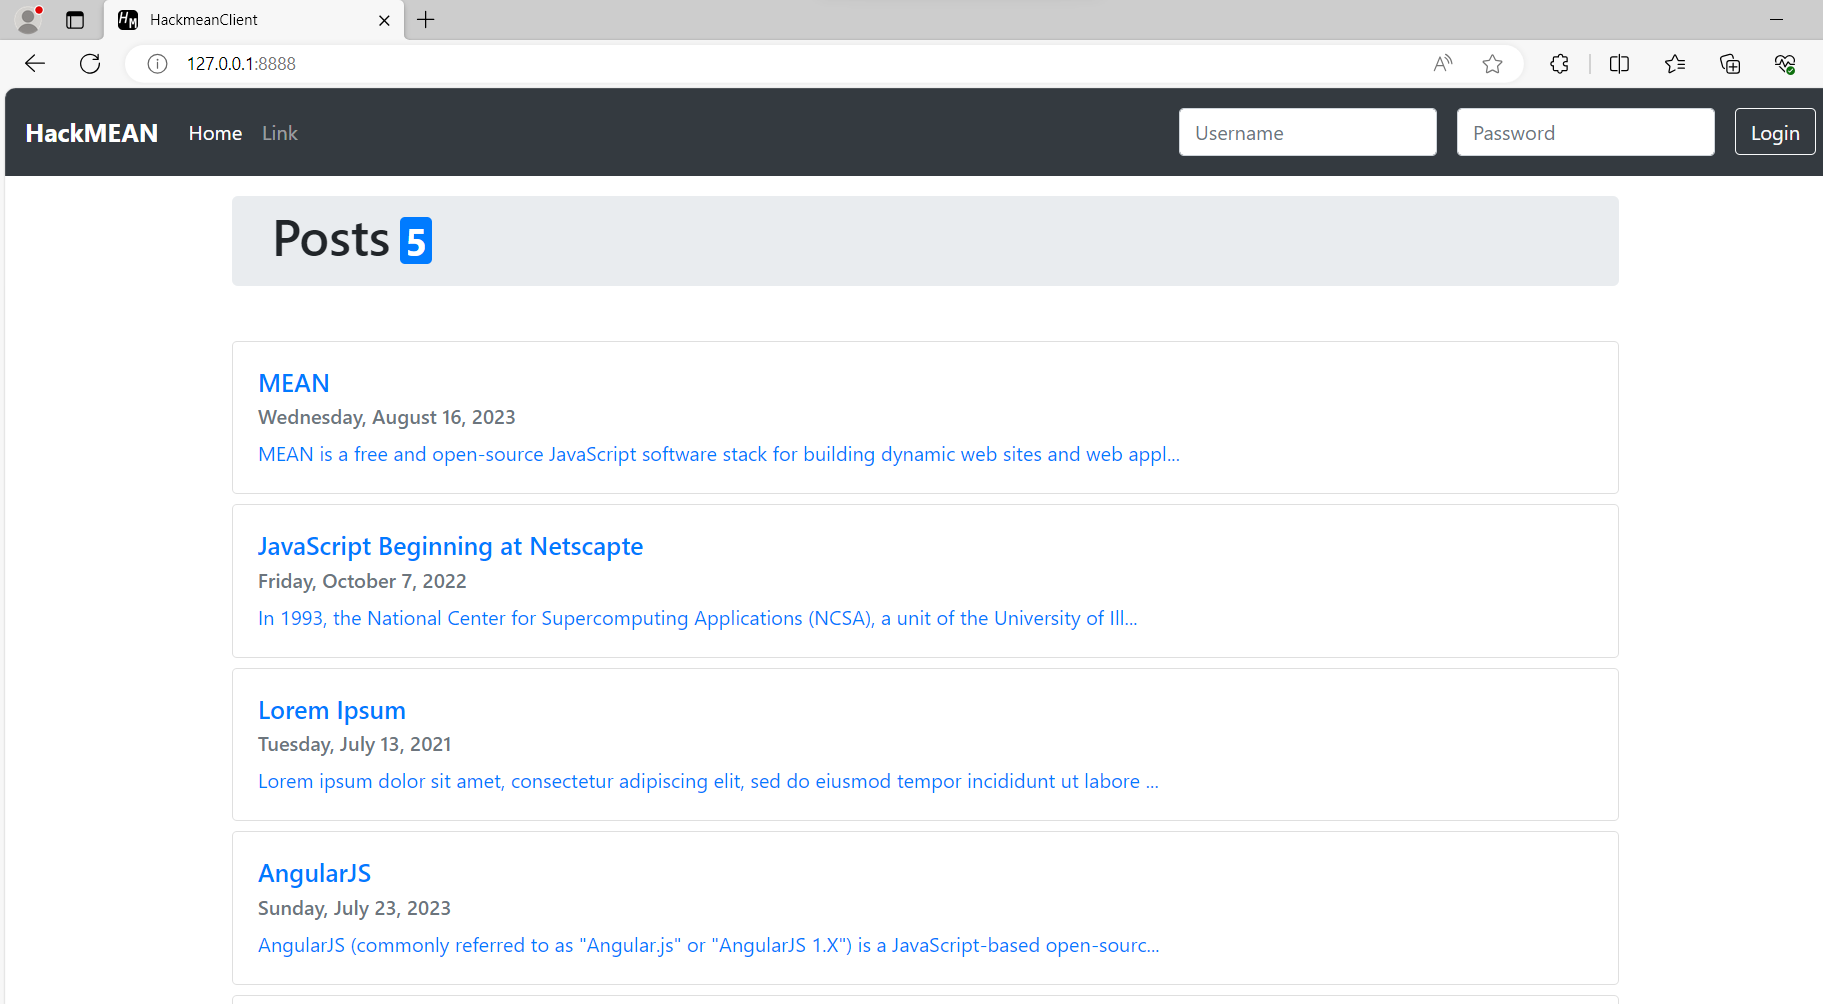
\includegraphics[scale=0.35]{Immagini/img20.png}}%
    \caption{Applicazione HackMEAN}
    \label{fig:HackMEAN}
\end{figure}
Con la visualizzazione del sito dell’applicazione possiamo ricavarne il link, che in seguito utilizzeremo per effettuare una scansione automatizzata su OWASP zap.
\begin{figure}[H]
    %centrare senza margini
    \makebox[\textwidth][c]{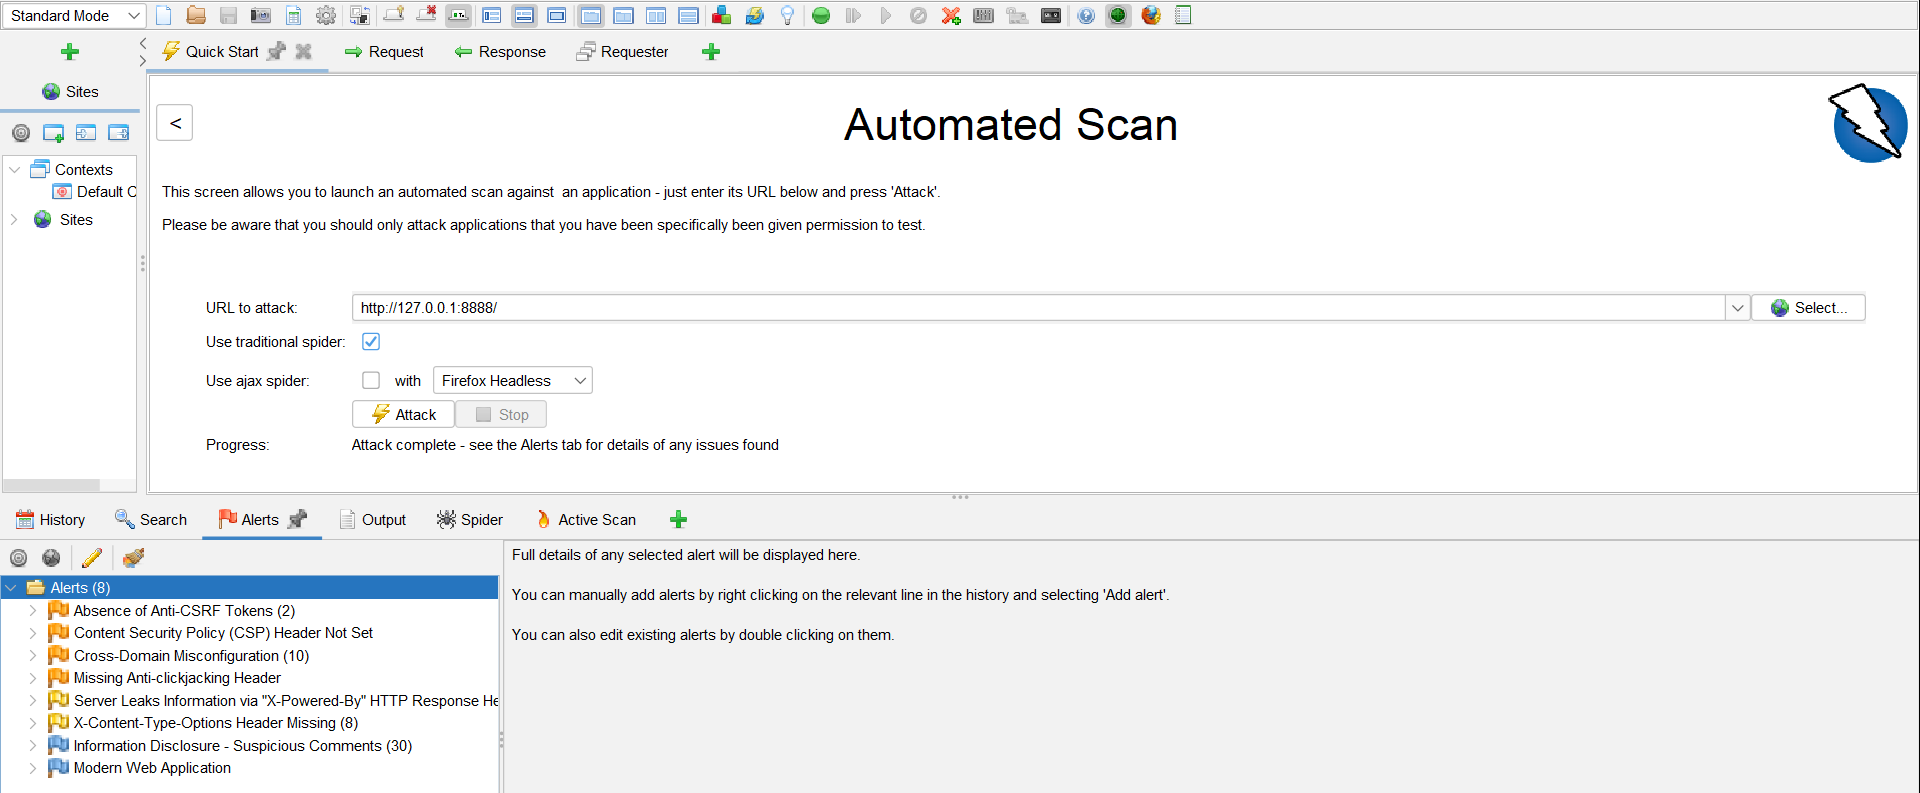
\includegraphics[scale=0.35]{Immagini/img22.png}}%
    \caption{Scanner HackMEAN}
    \label{fig:HackMEANScan}
\end{figure}
In basso a sinistra si trovano la lista di vulnerabilità trovate, dalla più grave alla meno grave, e selezionandole si potrà osservare la sua descrizione ed i modi per sanarla.
Per generare il report dell’analisi effettuata si dovrà cliccare sul pulsante in alto a destra e si otterrà in maniera automatica un report. 
Ecco la visualizzazione delle vulnerabilità all’interno del report:

\begin{figure}[H]
    %centrare senza margini
    \makebox[\textwidth][c]{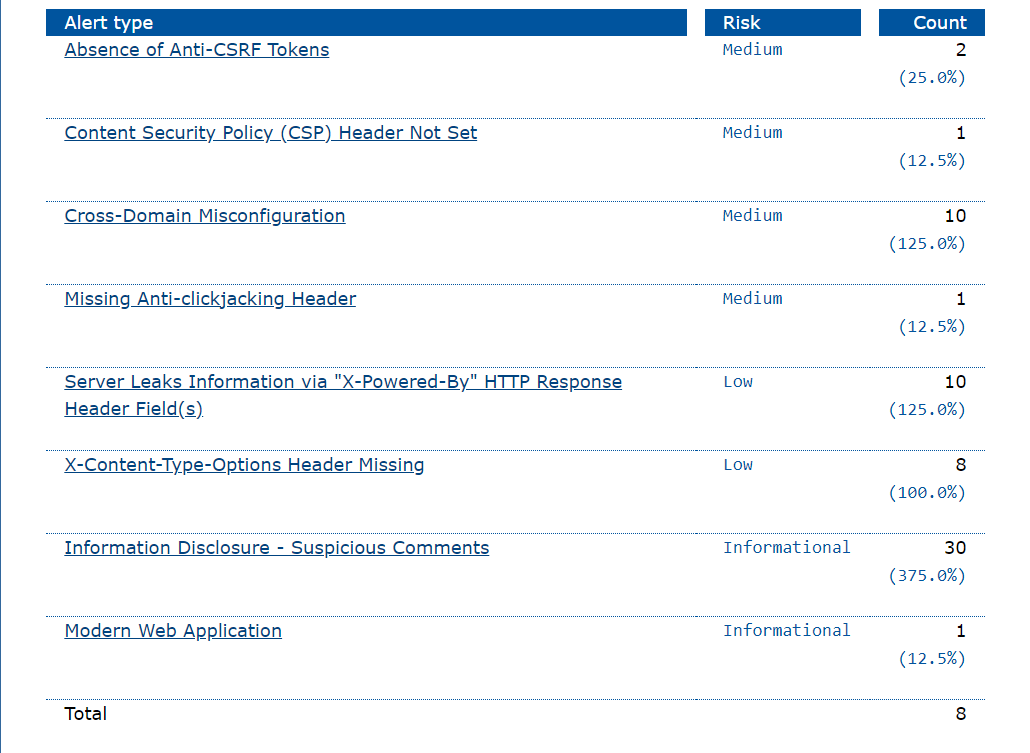
\includegraphics[scale=0.55]{Immagini/img21.png}}%
    \caption{Report HackMEAN }
    \label{fig:reportHackMEAN}
\end{figure}

Come possiamo osservare non sempre nei report vengono riportate vere e proprie vulnerabilità ma spesso si trovano potenziali forme di pericolo, facilmente attaccabili e quindi segnalate dal report.
Questo è solo un indice dei pericoli trovati, all’interno dell’intero report queste minacce verranno analizzate maggiormente nel dettaglio, descrivendo la vulnerabilità e come risolverla, inserendo riferimenti validi alla documentazione del problema stesso.
Di seguito alla generazione del report è opportuno testare manualmente le vulnerabilità trovate. 


\section{Cloud Computing} 
Le aziende stanno sfruttando il Cloud come fattore chiave per completare la trasformazione digitale e la pandemia di COVID ha ulteriormente accelerato questa tendenza. Il cloud sta diventando uno dei principali punti all’ordine del giorno dei dirigenti poiché le aziende stanno passando da un approccio frammentario a una trasformazione digitale end-to-end più olistica con il cloud al centro. 
Quando si supera un determinato limite di storage e utilizzo dei dati perché l’azienda sta attraversando una fase di espansione, solitamente ci si affida a un sistema di server che funziona su hardware sarai costretto, prima o poi, a modificarne una parte o a sostituirli completamente, con tutte le spese connesse.
Se, invece, si opta per una gestione dei dati su Cloud, si può scegliere di aumentare lo spazio a disposizione senza incidere sugli investimenti in beni materiali, che pesano sul bilancio annuale in quantità notevole e possono rappresentare un freno allo sviluppo armonico dell’azienda, sia al suo interno che all’esterno. 
Il Cloud computing rappresenta una valida soluzione che aiuta tutte le aziende a crescere in modo sano, indipendentemente dalle dimensioni e dal fatturato, perché contribuisce a diffondere un clima di trasparenza, condivisione e collaborazione.
Il Cloud aiuta le aziende a crescere e a svilupparsi, in particolare se si tratta di realtà piccole ma dinamiche e in forte sviluppo, un sistema di gestione condivisa e flessibile dei dati aziendali contribuisce a creare e mantenere ordine, sicurezza e competitività, con un abbassamento dei costi, al contrario per imprese medio-grandi  l’adozione del Cloud Computing consente l’elaborazione e condivisione in tempo reale di un’ingente quantità di dati e informazioni, con la massima sicurezza e attraverso una struttura di autorizzazioni e permessi che controllano in modo automatico gli accessi.
\subsection{Cos’è il Cloud Computing} 
Il termine cloud indica una rete di server che si trovano in Data Center sparsi per il mondo al quale è possibile accedere tramite internet. I Data Center permettono di usufruire di risorse, strumenti e servizi direttamente online.  Il cloud, quindi, non può essere definito un’entità fisica, piuttosto si tratta di un’ampia rete di server remoti e connessi tra di loro e progettati per lavorare come un unico ecosistema. 
Il cloud, e la sua definizione, si basano su 3 concetti principali:
\begin{itemize}
    \item la fornitura di servizi di archiviazione ed elaborazione
    \item grazie alla virtualizzazione, la condivisione della stessa risorsa informatica da parte di più persone
    \item l’accessibilità ai dati per mezzo della rete informatica
\end{itemize}
Nel cloud computing, ogni server è connesso all’altro, creando così una rete globale di servizi accessibili da qualsiasi dispositivo connesso alla rete. Il cloud viene rappresentato con una nuvola proprio perché i dati sono sparsi in diversi data center, come se vivessero in una nuvola virtuale.
\subsection{Evoluzione del Cloud Computing} 
\cite{storia_cloud}
Si tratta di un concetto le cui radici risalgono agli anni Sessanta e che con il passare del tempo è mutato. Non solo per via del progresso tecnologico, ma anche per gli obiettivi.All’inizio non vi era una vera e propria definizione, né una parola che potesse racchiudere questo concetto mutato con il passare del tempo. Tra la fine degli anni ’60 e durante il seguente decennio, si iniziò a parlare di “time-sharing”, ovvero l’utilizzo simultaneo di grandi unità centrali (mainframe) da parte di un numero elevato (non come oggi) di utenti che potevano accedere ai pc in remoto, dai propri dispositivi.
Questa, dunque, è stata la base storica che ci aiuta a capire cos'è un Cloud. Il primo grande passo in avanti è arrivato tra gli anni ’80 e ’90, quando grazie all’inizio della diffusione di pc e di internet, le principali aziende del settore hanno iniziato a realizzare e rendere fruibili i primi servizi di hosting: con questi, i clienti che acquistavano questo prodotto informatico, erano in grado di archiviare i dati sui server remoti di terze parti. Dunque, in questi anni il concetto di Cloud ebbe un grande impulso verso lo sviluppo.
Tra la fine degli anni ’90 e i primi anni 2000, il Cloud iniziò a diventare uno strumento utilizzato su larga scala, mutando anche alcuni dettagli del suo significato originale: da allora, infatti, questo termine ha iniziato a indicare la fornitura di servizi e risorse informatiche attraverso Internet. Non solo, dunque, archiviazione, ma anche un’altra serie di funzionalità utili per la gestione dei servizi informatici privati. E non è un caso che nel 2006 Amazon immise sul mercato il suo AWS (Amazon Web Services), un servizio in grado di fornire non solo i principi basilari del cloud computing (ovvero l’archiviazione di dati personali), ma anche funzioni di calcolo e di database rivolti ad aziende e sviluppatori. Da quel momento, moltissime altre aziende Big Tech hanno iniziato a investire e sviluppare i propri sistemi di Cloud Computing, creando una vera e propria contesa commerciale. Subito dopo Amazon, infatti, anche Google lanciò il proprio servizio (Google Cloud Platform), seguito da Microsoft che ha puntato tutto su Azure. Oggi,il panorama commerciale attorno al Cloud si è arricchito di numerosi attori.
\subsection{Modelli di distribuzione del Cloud Computing}
\begin{itemize}
    \item Cloud pubblico: connettersi ad un cloud pubblico significa utilizzare una connessione Internet per accedere alle risorse informatiche ospitate su data center gestiti da un fornitore di servizi cloud di terze parti, anziché possedere e mantenere tali risorse in sede. Un cloud pubblico condiviso prevede che molte organizzazioni (o tenant) condividano la stessa infrastruttura.
    \item Cloud privato: questo modello cloud è ottimo per le organizzazioni preoccupate di condividere le risorse su un cloud pubblico. È implementato su server di proprietà e gestiti dall'organizzazione e vi si accede tramite Internet o tramite una rete interna privata.
    \item Cloud ibrido: molte organizzazioni utilizzano effettivamente una combinazione di diversi ambienti cloud. Questo viene definito approccio cloud ibrido. Il cloud ibrido spesso include una combinazione di cloud pubblico e cloud privato, spesso in combinazione con alcune infrastrutture locali.
    \item Multi-cloud: un approccio multi-cloud è un caso particolare di cloud ibrido in cui un'organizzazione utilizza servizi di più provider di cloud pubblici. 
\end{itemize}
\subsection{Categorie di servizi del Cloud Computing}
\cite{servizi_cloud}
\begin{itemize}
\item Software as a Service (SaaS): SaaS è il servizio di applicazioni cloud più comunemente utilizzato e sta diventando il modo dominante per le organizzazioni di accedere alle applicazioni software.Con SaaS, un'organizzazione accede a un'applicazione software specifica ospitata su un server remoto e gestita da un provider di terze parti. In base all'abbonamento, l'accesso all'applicazione avviene tramite un browser Web, riducendo la necessità di download o aggiornamenti del software sul dispositivo. I prodotti SaaS più diffusi includono  Salesforce ,  Workday o  Microsoft Office 365 .
\item Platform as a Service (PaaS): PaaS è una scelta popolare per le aziende che desiderano creare applicazioni uniche senza effettuare importanti investimenti finanziari.Con PaaS, un'organizzazione accede a un ambiente predefinito per lo sviluppo software che può essere utilizzato per creare, testare ed eseguire applicazioni. Ciò significa che gli sviluppatori non devono iniziare da zero durante la creazione di app. PaaS consente allo sviluppatore di concentrarsi sul lato creativo dello sviluppo del software, anziché su attività noiose come la scrittura di codici estesi o la gestione degli aggiornamenti software o delle patch di sicurezza. Esempi di prodotti PaaS includono Google App Engine, server Web e server SQL.
\item Infrastructure as a Service (IaaS): IaaS è l'opzione più semplice per le aziende. Con IaaS, un'organizzazione migra il proprio hardware, noleggiando server e storage di dati nel cloud anziché acquistare e mantenere la propria infrastruttura.
IaaS fornisce a un'organizzazione le stesse tecnologie e funzionalità di un data center tradizionale, incluso il controllo completo sulle istanze del server. Gli amministratori di sistema all'interno dell'azienda sono responsabili della gestione di aspetti quali database, applicazioni, runtime, sicurezza, ecc., mentre il fornitore di servizi cloud gestisce server, dischi rigidi, rete, archiviazione, ecc.
\end{itemize}
\subsection{Vantaggi del Cloud Computing}
\cite{vantaggi_cloud}
Le aziende dovrebbero scegliere il Cloud perché questo strumento costituisce la soluzione a molte delle problematiche interne e delle sfide poste dall’esterno che tutte le imprese affrontano nella loro attività quotidiana.

Ecco illustrati alcuni dei vantaggi Cloud:
\begin{itemize}
    \item Flessibilità e risparmio: gli investimenti in infrastrutture informatiche e hardware rappresentano un peso rilevante nel bilancio di un’impresa, che oltre alla spesa iniziale o periodica per l’acquisto di attrezzature quali server e client affronta l’ammortamento annuale dei macchinari, soggetti a una veloce obsolescenza. Se, al contrario, si utilizza un sistema di gestione dei dati aziendali tramite Cloud, verrà sostenuto solo il costo legato alla quantità di spazio virtuale e dati che ti servono, con la possibilità di modificare il piano prescelto quando ne hai la necessità. Con l’utilizzo del sistema Cloud si usufruisce di un servizio efficace dai costi prevedibili, ricorrenti e frazionabili su base mensile e che, oltretutto, sono imputati a costi per servizi e non per immobilizzazioni materiali.
    \item Maggiore sicurezza: un altro vantaggio del Cloud per le aziende riguarda la garanzia di un livello di sicurezza molto elevato nella protezione dei dati. Il rischio di cybercriminalità e furti di identità sono tutt’altro che un’eventualità, soprattutto nelle reti aziendali.Tutti i dati e le informazioni salvate sul Cloud sono memorizzate all’interno di più server dislocati, di conseguenza, è improbabile che tutti questi server vengano attaccati contemporaneamente.
    \item Maggiore produttività: Il Cloud offre alle piccole e medie imprese strumenti tecnologici che queste non potrebbero affrontare, in termini quantitativi e qualitativi. L’ampia gamma di servizi del Cloud, dalla gestione dello spazio di storage a quella delle autorizzazioni interne di accesso ai dati, è altamente sofisticata, complessa e prevede team dedicati al continuo sviluppo e aggiornamento di applicativi ad hoc. Anche a livello di macro pensiero e sviluppo della cultura aziendale, il Cloud costituisce un cambiamento radicale, perché la logica di condivisione dei documenti, da parte dei collaboratori, in un unico archivio virtuale presuppone un salto di qualità nell’approccio al teamworking, contribuendo alla costruzione e al consolidamento di una solida cultura di impresa.
\end{itemize}
\subsection{Gestione delle vulnerabilità in applicazioni Cloud}
\cite{gestione_vulnerabiltà}
La gestione delle vulnerabilità nel cloud computing può essere definita come un approccio o processo continuo volto a identificare, analizzare, dare priorità e risolvere i problemi di sicurezza nel cloud computing.
Non solo riduce al minimo eventuali rischi per la sicurezza correggendo le vulnerabilità comuni, ma garantisce anche che tutte le lacune di sicurezza attraverso le quali gli aggressori possono entrare nel framework siano adeguatamente bloccate.
È diventato un pilastro fondamentale nelle moderne minacce alla sicurezza del cloud poiché rileva attivamente tutte le minacce e le risolve in modo efficace. Il cloud computing moderno è così vasto e complesso che componenti come dispositivi IoT, firewall di configurazione e contenitori di carichi di lavoro potrebbero causare problemi di sicurezza.
\subsection{Vulnerabilità comuni in applicazioni Cloud}
\begin{itemize}
    \item Configurazione errata nei contenitori: Una delle vulnerabilità più comuni è un’errata configurazione dei container che ha portato a gravi violazioni della piattaforma cloud.
    Queste configurazioni errate sono problemi che si sono verificati a causa della mancanza delle impostazioni sicure richieste o dell'accesso pubblico alla piattaforma cloud. L'errata configurazione del gruppo di sicurezza è un altro tipo di vulnerabilità che si verifica in un sistema di sicurezza e porta all'accesso diretto alla piattaforma cloud.
    \item Autenticazione impropria:Un processo di autenticazione inadeguato nel sistema di sicurezza cloud è un’altra vulnerabilità comune che spesso porta a violazioni della sicurezza. La mancanza di autenticazione a più fattori e la scarsa sicurezza della password rappresentano alcune gravi sfide nella gestione delle vulnerabilità del cloud.
    Inoltre, in assenza di un adeguato controllo degli accessi, qualsiasi utente autorizzato a cui non dovrebbe essere consentito l'accesso potrebbe riuscire ad accedere al sistema cloud.
    \item Inadempienza: La non conformità agli standard di settore come PCI-DSS, HIPAA, ISO 27001 e SOC 2 è una delle principali cause di vulnerabilità nella piattaforma cloud. Queste policy di gestione delle vulnerabilità cloud garantiscono che il carico di lavoro cloud sia adeguatamente protetto.
    Quando il fornitore di sicurezza cloud e il cliente gestiscono in modo improprio le impostazioni di sicurezza, si verificano problemi e gli aggressori ne approfittano per ottenere l’accesso al server. 
    \item Configurazione di rete errata: È fondamentale che la rete cloud sia configurata adeguatamente; in caso contrario, rischierebbe la sicurezza dei dati. Il team di sicurezza dovrebbe fare attenzione nel fornire l'accesso alla porta delle reti private perché se viene lasciata aperta per impostazione predefinita, chiunque può accedere ai dati sensibili.Il team di sicurezza dovrebbe fornire l'accesso alle porte specifiche necessarie per l'accesso e tutte le altre porte dovrebbero essere disabilitate per la connessione alle reti private.
    \item Scarsa gestione degli accessi ai dati sensibili: le piattaforme Cloud contengono molte applicazioni specifiche che possono aiutare chiunque ad accedere a molti dati accessibili. Pertanto è fondamentale non creare mai credenziali o ID di gruppo per tutte le applicazioni. Sarebbe l’ideale creare credenziali specifiche per applicazioni specifiche in cui solo il personale autorizzato potrà accedere.
    \item API protette in modo improprio: le API non sicure rappresentano uno dei modi principali con cui gli aggressori possono accedere alle piattaforme Cloud e rubare tutti i dati essenziali.  Gli aggressori cercano sempre API prive di autorizzazione e autenticazione adeguate e le sfruttano per scopi illeciti. 
\end{itemize}
\subsection{Funzionalità che rendono importante la gestione delle vulnerabilità del Cloud}
\begin{itemize}
    \item Protezione di sicurezza ottimale: la gestione delle vulnerabilità del Cloud è responsabile del monitoraggio e del rilevamento delle minacce del tuo sistema. Garantiscono che tutti i dati e le applicazioni siano completamente protetti, l’obiettivo è identificare le minacce e risolverle in maniera efficiente.
    \item Prevenzione efficace: misure preventive efficaci in modo che qualunque sia l'intensità dell'attacco diretto alla tua applicazione cloud e ai tuoi dati cruciali, la correzione delle vulnerabilità del cloud può facilmente prevenirli e bloccarli.
    \item Efficacia dei costi:Il monitoraggio, la gestione e il rilevamento manuale delle minacce nell'infrastruttura cloud sono attività costose e ingombranti, per questo con il monitoraggio costante e la rapida risoluzione delle minacce, la gestione delle vulnerabilità del cloud ti evita costi e perdite colossali nel caso in cui l'infrastruttura venga sfruttata.
    \item Risparmia tempo: quando i tuoi dati e le tue applicazioni nel cloud vengono monitorati dalla gestione delle vulnerabilità del cloud, puoi risparmiare molto tempo. 
\end{itemize}
\subsection{Pratiche di gestione delle vulnerabilità del Cloud}
\begin{itemize}
    \item Scansione costante delle vulnerabilità del cloud: utilizzare la capacità di scansione continua delle vulnerabilità del cloud per scansionare e rilevare le vulnerabilità nella loro fase iniziale. Questi scanner dovrebbero essere supportati da un elenco completo e aggiornato di vulnerabilità in modo che sia in grado di rilevare le minacce al loro livello precedente.Per una migliore efficacia, lo scanner dovrebbe essere in grado di rilevare eventuali errori logici, accantonare eventuali falsi positivi e avviare la scansione dell'accesso.
    \item Test di penetrazione sistematico: eseguire test di penetrazione aiuta ad eseguire scansioni approfondite in cui si analizza la vulnerabilità ed il danno che può verificarsi in caso di attacchi.
    \item Scansione delle vulnerabilità durante l’integrazione: l’utilizzo della scansione continua durante la fase di sviluppo di un’applicazione è un modo per mantenere una protezione completa.
\end{itemize}

